% AJ,APJ copyright persmissions: https://journals.aas.org/article-charges-and-copyright/#AAS_material
% MNRAS copyright permissions https://academic.oup.com/mnras/pages/rights_and_new_business_development
% A&A email to (e-mail: aanda.paris@obspm.fr)

%%%%%%%%%%%%%%%%%%%% author.tex %%%%%%%%%%%%%%%%%%%%%%%%%%%%%%%%%%%
%
% Template for the Handbook of X-ray and Gamma-ray Astrophysics (preliminary version)
%
%%%%%%%%%%%%%%%% Springer %%%%%%%%%%%%%%%%%%%%%%%%%%%%%%%%%%
\documentclass[graybox, nosecnum]{svmult}

% choose options for [] as required from the list
% in the Reference Guide

\usepackage{mathptmx}       % selects Times Roman as basic font
\usepackage{helvet}         % selects Helvetica as sans-serif font
\usepackage{courier}        % selects Courier as typewriter font
\usepackage{type1cm}        % activate if the above 3 fonts are
                            % not available on your system
%
\usepackage{amssymb}
\usepackage{makeidx}         % allows index generation
\usepackage{graphicx}        % standard LaTeX graphics tool
                             % when including figure files
\usepackage{multicol}        % used for the two-column index
\usepackage[bottom]{footmisc}% places footnotes at page bottom
\usepackage{hyperref}        %for hyperlinks
\usepackage{soul}            % for high-lighting of text
\hypersetup{colorlinks=true,urlcolor=blue}
%
\usepackage[square,numbers]{natbib}
%\bibliographystyle{ieeetr}
\newcommand{\hbindex}[1]{\hl{#1}\index{#1}}  %highlights index entries
\makeindex             % used for the subject index
                       % please use the style svind.ist with
                       % your makeindex program
%%%%%%%%%%%%%%%%%%%%%%%%%%%%%%%%%%%%%%%%%%%%%%%%%%%%%%%%%%%%%%%%%%%%%%%%%%%%%%%%%%%%%%%%%

% List of common astronomy symbols we use throughout
\usepackage{xspace}

\newcommand{\sun}{$_{\odot}$\xspace}

\DeclareRobustCommand{\ion}[2]{%
\relax\ifmmode
\ifx\testbx\f@series
{\mathbf{#1\,\mathsc{#2}}}\else
{\mathrm{#1\,\mathsc{#2}}}\fi
\else\textup{#1\,{\mdseries\textsc{#2}}}%
\fi}

\def\degr{\hbox{$^\circ$}}
\def\arcmin{\hbox{$^\prime$}}
\def\arcsec{\hbox{$^{\prime\prime}$}}
\def\utw{\smash{\rlap{\lower5pt\hbox{$\sim$}}}}
\def\udtw{\smash{\rlap{\lower6pt\hbox{$\approx$}}}}
\def\fd{\hbox{$.\!\!^{\rm d}$}}
\def\fh{\hbox{$.\!\!^{\rm h}$}}
\def\fm{\hbox{$.\!\!^{\rm m}$}}
\def\fs{\hbox{$.\!\!^{\rm s}$}}
\def\fdg{\hbox{$.\!\!^\circ$}}
\def\farcm{\hbox{$.\mkern-4mu^\prime$}}
\def\farcs{\hbox{$.\!\!^{\prime\prime}$}}


\def\aj{AJ}%

          % Astronomical Journal

\def\araa{ARA\&A}%

          % Annual Review of Astron and Astrophys

\def\apj{ApJ}%

          % Astrophysical Journal

\def\apjl{ApJ}%

          % Astrophysical Journal, Letters

\def\apjs{ApJS}%

          % Astrophysical Journal, Supplement

\def\ao{Appl.~Opt.}%

          % Applied Optics

\def\apss{Ap\&SS}%

          % Astrophysics and Space Science

\def\aap{A\&A}%

          % Astronomy and Astrophysics

\def\aapr{A\&A~Rev.}%

          % Astronomy and Astrophysics Reviews

\def\aaps{A\&AS}%

          % Astronomy and Astrophysics, Supplement

\def\azh{AZh}%

          % Astronomicheskii Zhurnal

\def\baas{BAAS}%

          % Bulletin of the AAS

\def\jrasc{JRASC}%

          % Journal of the RAS of Canada

\def\memras{MmRAS}%

          % Memoirs of the RAS

\def\mnras{MNRAS}%

          % Monthly Notices of the RAS

\def\pra{Phys.~Rev.~A}%

          % Physical Review A: General Physics

\def\prb{Phys.~Rev.~B}%

          % Physical Review B: Solid State

\def\prc{Phys.~Rev.~C}%

          % Physical Review C

\def\prd{Phys.~Rev.~D}%

          % Physical Review D

\def\pre{Phys.~Rev.~E}%

          % Physical Review E

\def\prl{Phys.~Rev.~Lett.}%

          % Physical Review Letters

\def\pasp{PASP}%

          % Publications of the ASP

\def\pasj{PASJ}%

          % Publications of the ASJ

\def\qjras{QJRAS}%

          % Quarterly Journal of the RAS

\def\skytel{S\&T}%

          % Sky and Telescope

\def\solphys{Sol.~Phys.}%

          % Solar Physics

\def\sovast{Soviet~Ast.}%

          % Soviet Astronomy

\def\ssr{Space~Sci.~Rev.}%

          % Space Science Reviews

\def\zap{ZAp}%

          % Zeitschrift fuer Astrophysik

\def\nat{Nature}%

          % Nature

\def\iaucirc{IAU~Circ.}%

          % IAU Cirulars

\def\aplett{Astrophys.~Lett.}%

          % Astrophysics Letters

\def\apspr{Astrophys.~Space~Phys.~Res.}%

          % Astrophysics Space Physics Research

\def\bain{Bull.~Astron.~Inst.~Netherlands}%

          % Bulletin Astronomical Institute of the Netherlands

\def\fcp{Fund.~Cosmic~Phys.}%

          % Fundamental Cosmic Physics

\def\gca{Geochim.~Cosmochim.~Acta}%

          % Geochimica Cosmochimica Acta

\def\grl{Geophys.~Res.~Lett.}%

          % Geophysics Research Letters

\def\jcp{J.~Chem.~Phys.}%

          % Journal of Chemical Physics

\def\jgr{J.~Geophys.~Res.}%

          % Journal of Geophysics Research

\def\jqsrt{J.~Quant.~Spec.~Radiat.~Transf.}%

          % Journal of Quantitiative Spectroscopy and Radiative Trasfer

\def\memsai{Mem.~Soc.~Astron.~Italiana}%

          % Mem. Societa Astronomica Italiana

\def\nphysa{Nucl.~Phys.~A}%

          % Nuclear Physics A

\def\physrep{Phys.~Rep.}%

          % Physics Reports

\def\physscr{Phys.~Scr}%

          % Physica Scripta

\def\planss{Planet.~Space~Sci.}%

          % Planetary Space Science

\def\procspie{Proc.~SPIE}%

          % Proceedings of the SPIE

\let\astap=\aap

\let\apjlett=\apjl

\let\apjsupp=\apjs

\let\applopt=\ao

%

\uchyph=0


\begin{document}
%\tableofcontents{}
\title*{Pre main sequence:  Accretion \& Outflows}
% Use \titlerunning{Short Title} for an abbreviated version of
% your contribution title if the original one is too long
\author{Christian P. Schneider  \thanks{corresponding author}, H. Moritz G\"unther, and Sabina Ustamujic}
% Use \authorrunning{Short Title} for an abbreviated version of
% your contribution title if the original one is too long
\institute{Christian P. Schneider \at Hamburg Observatory, Gojenbergsweg 11, 21029 Hamburg, Germany, \email{christian.schneider@hs.uni-hamburg.de}
\and H. Moritz G\"unther \at Kavli Institute for Astrophysics and Space Research, Massachusetts Institute of Technology,
77 Massachusetts Avenue, Cambridge, MA 02139, USA \email{hgunther@mit.edu}
\and S. Ustamujic \at Institute 2, Address of Institute 2 \email{sabina.ustamujic@inaf.it}}
%
% Use the package "url.sty" to avoid
% problems with special characters
% used in your e-mail or web address
%
\maketitle
%
\abstract{Each chapter should be preceded by an abstract (about 250 words) that summarizes the content. The abstract will appear \textit{online} at \url{www.SpringerLink.com} and be available with unrestricted access. This allows unregistered users to read the abstract as a teaser for the complete chapter. Please do not include reference citations, cross-references or undefined abbreviations in the abstract.}
\section{Keywords}
Please provide keywords required to facilitate search of chapter on web; maximum 10 keywords.


\section{Introduction {\normalfont (3 pages) [Christian]}}

``The fundamental problem of star formation is how stars accrete their mass.'' \citep{Dunham_2014}.


How did the Sun form, how the Earth? Answering these questions requires the identification and study of the Sun's progenitors,  young stellar objects that will evolve into a stellar system like ours. Therefore, we primarily discuss stellar systems broadly resembling the young Sun's, i.e., with stellar masses below about 2$\,M_\odot$.

Such stars and planets form in molecular clouds, often associated with filaments within the clouds,  where denser, cooler parts collapse. In these regions, gravity dominates over the stabilizing effects of thermal pressure, turbulence, and magnetic fields \citep[e.g., ][]{McKee_2007} and protostars form  \citep{Andre_2014}. The first, self-gravitating, hydrostatic core contains only a small fraction of the final stellar mass ($\sim0.01\,M_\odot$) and most of the mass still in the envelope \citep[e.g.,][]{Gong_2015,Lee_2020}; these objects are called class~0 objects \citep[see Fig.~\ref{fig:starform_classes} top left, and ][]{Andre_1993, Larson_2003}. Due to angular momentum conservation, a disk forms around the central condensation and outflows are launched, which regulate the angular momentum balance of the system. The collimated outflows, jets, propagate into the interstellar medium beyond the envelope and are often the first detectable signs of a forming star. After disk formation, accretion proceeds through the disk onto the protostar while enevelope material falls onto the disk \citep{Padoan_2014}. Eventually, the protostar's mass equals the envelope mass after roughly $10^5$\,yrs and the objects are called class~{\sc i} objects (Fig.~\ref{fig:starform_classes} top right), they are also hotter and more luminous than class~0 objects. It is believed that planet formation sets in during the class~I stage \citep{}.

Eventually, the envelope disperses and the young stellar object (YSO) becomes visible at optical wavelengths at a stellar age of $\sim1\,$Myr. The dispersal mechanism is not clear yet, but winds and radiation from nearby OB stars if present or otherwise radiation and outflows from low mass stars likely play a major role. Also the (wide-angle) winds launched by the forming stellar system itself may contribute to the envelope dispersal and to reduce the envelope to star mass conversion efficiency of to one third \citep{Frank_2014}. Accretion then proceeds from the disk in these class~{\sc ii} sources or classical T~Tauri stars. Planet formation is already ongoing during this stage of star formation and we get a first relatively unobscured view to the newborn stars (Fig.~\ref{fig:starform_classes} bottom left).

\begin{figure}[t]
\centering
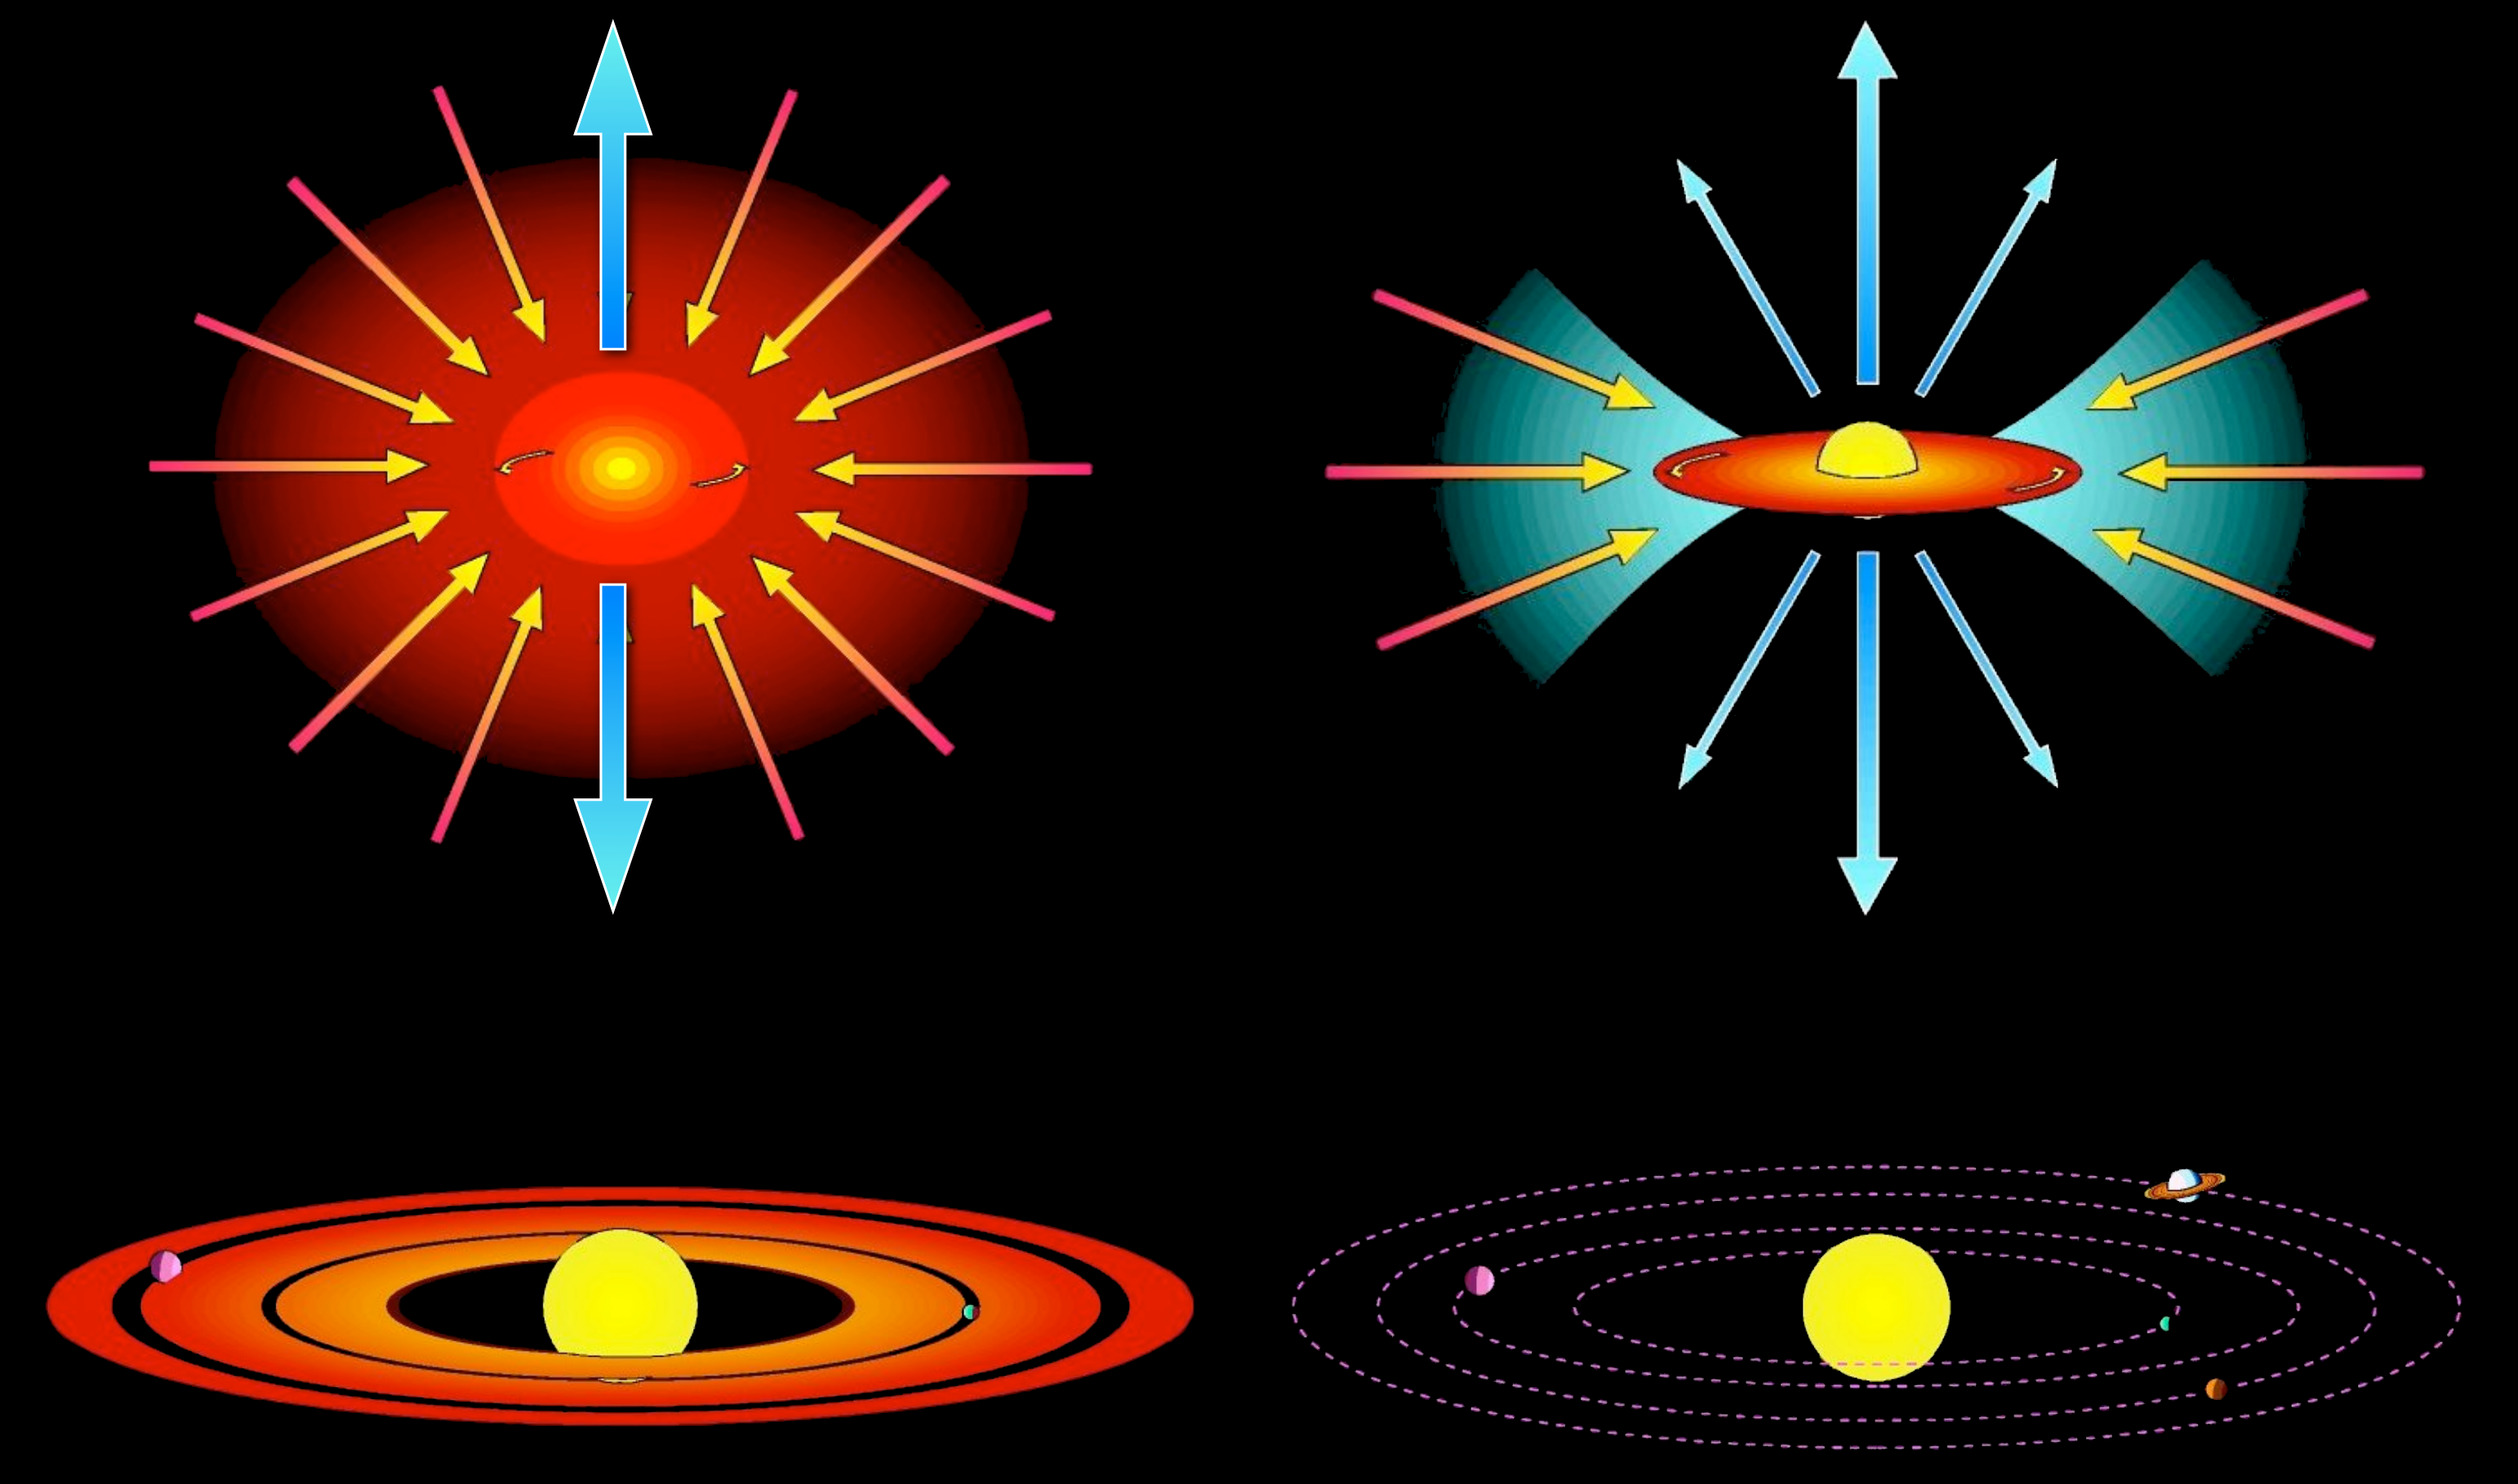
\includegraphics[width=10cm]{figs/starform_classes.png}
\caption{Star formation sequence. Adapted from original diagram by M.~McCaughrean. \label{fig:starform_classes}}
\end{figure}

Finally, the disk dispersed, too, after another few Myrs leaving behind a pre-main sequence star, perhaps surrounded by planetary system, which slowly contracts towards it's  main-sequence radius (Fig.~\ref{fig:starform_classes} bottom right). Solar mass stars take approximately 100\,Myrs to reach the main sequence where they reside for over 10\,Gyr.

Within this sequence of star formation, the classical T~Tauri star phase stands out, because the relatively unobscured view towards the central region around the forming stars provides us with the most detailed picture of the physical processes, including planet formation, using a large variety of observational techniques including X-ray data.

\subsection{T Tauri Stars}
T~Tauri stars were first described as a distinct class of objects  by \citeauthor{Joy_1945} in 1945 based on their pronounced optical variability \citep{Joy_1945}. The notation that T~Tauri stars are young came with the realization that they are located to the top right of  main sequence (MS) stars in the Hertzsprung-Russel diagram (HRD), consistent with the expected position of stars contracting along their Hayashi tracks towards the MS \citep{Hayashi_1961}. Also , strong Li absorption lines suggest a young age, because  Li is quickly depleted in stellar photospheres \citep{Magazzu_1992}.


\begin{figure}[t]
\centering
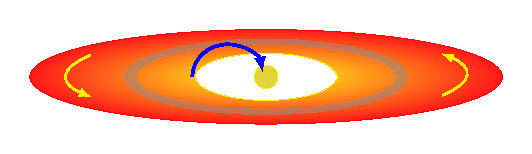
\includegraphics[width=10cm]{sketches/ctts.pdf}
\caption{Sketch of a classical T~Tauri system. \label{fig:ctts_sketch}}
\end{figure}


The physical processes that cause other prominent features seen in the so-called classical T~Tauri stars (CTTSs), however, remained controversial.
For example, there was no consensus on the origin of the
strong emission lines like H$\alpha$, termed “chromospheric emission”, until the 1980s when the infrared excess of CTTSs was discovered and correctly ascribed to cold dusty disks around the central star. Also, the discovery that the ``chromospheric'' line profiles change from inverse to normal P~Cygni profiles and back within few days on individual systems helped to converge on a scenario in which accretion shocks and outflows are the main processes for explaining CTTS features \citep[as nicely described in][]{Bertout_2007}, in addition to their protoplanetary disks.

Disks, accretion, and outflow are still the processes that define the properties of CTTS. Figure~\ref{} shows a sketch of a T Tauri system.
During the CTTS phase, the stellar mass is already close to the final stellar mass but the interior is fully convective \citep{}, which together with rather rapid rotation (few days) leads to a strong stellar dynamo \citep{}. Stellar magnetic fields during the CTTS phase are therefore in the kG range \citep{}. Such strong magentic fields disrupt the disk close to the star, that is within a few stellar radii, as the star, being hydrostatic, rotates slower than an approximately Keplerian disk. The interaction of the stellar magnetic field with the inner parts of the disk slows the innermost disk material down so that it cannot resist gravity anymore and is channeled along the stellar magentic field lines onto the star. Travelling along the magnetic field line, the matieral is accelerated to almost free-fall velocity and impacts the stellar photosphere where a strong shock forms. The details of the accretion shock are described in sect.~\ref{sect:accretion}.%, briefly the shock velocities are on the order of 300\,km\,s$^{-1}$ resulting in post shock temperatures in the $10^6$\,K range and, thus, radiative cooling of the post shock plasma causes X-ray emission.

The inner disk would be depleted within $10^3$ to $10^4$ years without being replenished by material from outer disk radii. Therefore, continued accretion requires radial transport of material through the disk, from outer to inner disk radii. Radial transport through the disk requires the redistribution of angular momentum (AM) and several processes have been invoke to promote this AM redistribution, prominent examples include the magneto-rational instability \citep[MRI,][]{Balbus_1991} with non-ideal MHD extensions and disk winds \citep{Blandford_1982, Pudritz_1983}, again with the inclusion of non-ideal MHD effects. In reality, the vertical structure of protoplanetary disks likely results in different transport mechanisms dominating at different disk heights with most of the mass being transported through the upper disk layers where also magnetro-centrifugally driven winds are launched.

Magneto-centrifugally launched winds require some net vertical magnetic field threading the disk. Material is accelerated along magnetic field lines until the magnetic field strength becomes insufficient to control the particle motion and the Lorentz force causes the collimation of the outflowing material into narrow jets. The jet velocity depends on the so-called magnetic lever arm, which relates the Keplerian velocity at the launch radius to the jet velocity and is of order 10 \citep{}; hence, jet velocities are on the order of 300\,km\,s$^{-1}$. In addition to disk winds, there may be other outflows like stellar winds, magneto-spheric ejections (from the star or the star-disk interaction region), or the so-called X-winds from the inner disk edge \citep{Shu_}. 

At some point, typically after a few Myrs, the disk has dispersed \citep{} and we are left with a pre-main sequence star with a number of orbiting planets, such objects are call weak-line T~Tauri stars (WTTSs). 

\subsection{The power of X-rays for studying T~Tauri stars}
The different parts of a classical T~Tauri system have grossly different temperatures: The disk midplane may be characterized by only few 10~K, the upper disk layers are likely above 1000~K, the inner edge of the disk is typically assumed to be around 2\,000~K, and we typical stellar photospheric temperatures are 3-4\,000~K. Therefore, the intrinsic emission of these different components peaks in very different wavebands, which is reflected in the observational tools used to study them, sub-mm radio to IR observations enjoy great popularity for disk studies while optical to NIR data are powerful for studying the more dynamic processes such as accretion and outflows. There are, however, some interesting exceptions, e.g., FUV data probe the hydrogen content of the inner disk as well as accretion \citep[see review by][]{Schneider_2020}.

On first sight, it may therefore appear surprising that X-ray observations play an important role for studying CTTS. However, a flow with velocities in excess of 300\,km\,s$^{-1}$, like the accretion flow or the jet, which rams into a stationary obstacle shock heats the post to temperatures in excess of 1\,MK  so that radiative cooling of such a plasma causes X-ray emission so that X-ray studies of CTTSs (and younger objects for the outflow case) probe the (in- and out-) flow properties. 

X-ray data is even powerful for studying disk properties using transmission spectroscopy. Extinction at optical wavelengths\footnote{Strictly radiation with wavelengths longer than the 912\,\AA{}, the Lyman limit of hydrogen.} is dominated by dust grains while X-rays are absorbed by gas and dust. The ratio of X-ray to optical extinction therefore depends on the absorber's gas-to-dust ratio, which has been beneficially used using transmission spectroscopy of near edge-on protoplanetary disks \citep{}. Lastly, T~Tauri stars are rapidly rotating and so are also strong X-ray emitters (see chapter by J.~Kastner).





\section{Accretion \label{sect:accretion}}
{\color{blue}(10 pages)}

Accretion is the defining characteristic of young stars. It is through accretion that they build up mass, it is through accretion that they accumulate angular momentum, and it is probably through magnetic connection between disk and accretion column that at least some part of their angular momentum is lost. Once accretions stops, the mass, chemical composition, and angular momentum of a star continue to evolve through winds, but on much longer time scales.

Today it is widely accepted that the accretion in T Tauri stars is magnetically funneled. The accretion disk does not reach down to the stellar surface. Instead, it is truncated at a few stellar radii where the inner edge of the disk co-rotates with the central star. While magnetic fields of young stars can be complex, at large distances the field will be dominated by a dipole component. Magnetic field lines couple to the inner disk and the disk material, ionized by the UV and X-ray radiation from the star, is forced to follow the field lines. As it falls in, gravity accelerates the matter to free-fall velocity until it hits the surface where a strong shock develops \cite{Shu_1994}. 

We first look at the accretion stream and the locations of the footpoints. Then, we describe the picture of simple-1D accretion shock  before we extend this to more detailed observations and models.

\subsection{The accretion stream and its foot points}
\label{sect:accretionsrteam}
The accretion stream is initially cool; it heats up as mass accelerates and comes close to the star. The most prominent tracers are the strong and complex hydrogen emission lines. In particular H$\alpha$ is usually optically thick, often shows red-shifted absorption components compatible with free-fall velocity \cite[e.g.][]{2000AJ....119.1881A}, and varies over time scales of hours \cite{dupree_2012}. Many emission lines do not vary with the stellar rotation period, indicating that it is the inner disk, not the anchor point on the stellar surface, that controls the geometry of accretion \cite{2021A&A...649A..68S}.

Zeeman-Doppler imaging can reveal the structure of the magnetic field and, using certain assumptions, those fields can be extrapolated out to the inner disk edge. There seems to be an evolution of magnetic field strength and geometry, where the strength of the dipole component, which dominates the field at large radii and is thus most important for coupling to the accretion disk and carrying the accretion funnel, decreases with the depth of the convective envelope \cite{2012ApJ...755...97G,2019A&A...622A..72V}. On the stellar surface itself, Doppler imaging can locate the position of the accretion funnels which are often found near the pole, e.g.\ in BP Tau \cite{2008MNRAS.386.1234D} or V2129 Oph \cite{2011A&A...530A...1A}, but sometimes at lower latitudes as in V2247 Oph \cite{2010MNRAS.402.1426D}. Simulations can reproduce the analytical model of accretion foot points near the pole in the dipolar field, but they also point to more complex geometries when disk, stellar rotation, and stellar magnetic field are not aligned (Fig.~\ref{fig:romanova}).

\begin{figure}[t]
\centering
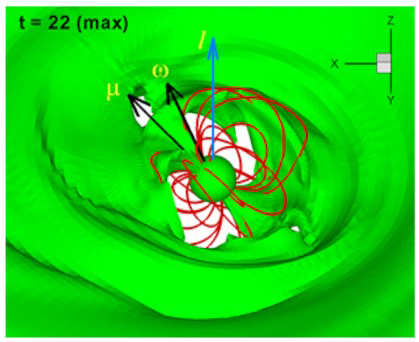
\includegraphics[width=5cm]{figs/Romanova2021fig8-panel.png}
\caption{Simulation of accretion on an inclined dipole. Mass flows towards the magnetic pole \cite{2021MNRAS.506..372R} \textcolor{blue}{need to ask for permission} \label{fig:romanova}}
\end{figure}

In one case, TW Hya, the signal is strong enough to determine the line shift of the soft X-ray lines to $38.3 \pm 5.1$~km/s \cite{2017A&A...607A..14A}. Since this is much less than the free-fall velocity, we must see the shock close perpendicular to the line-of-sight. TW~Hya is observed close to pole-on, so the accretion shocks must the located in the equatorial region.




\subsection{X-ray signatures of the accretion shock}
\label{sect:accretionobs}
{\color{blue}Moritz, Christian

Kastner & Brickhouse spectra, other spectra?, Argiroffi redshift? yes, Brickhouse 2012 variability,  naturepaper solar!, argiroffi V2129, V4046}


% Moritz list of citations to be put in the correct location later
AA Tau?

MHD modelin coal abs 2014ApJ...795L..34B 

2011A&A...526A.104C curran



The X-ray emission from cool stars on the main-sequence is caused by coronal activity. Young stars rotate faster and thus have more magnetic activity and stronger coronal X-rays than older stars such as our Sun. That is why accretion signatures are hard to find in broad-band X-ray spectra, in particular for stars embedded in a molecular cloud. To the contrary, surveys even show reduced X-ray flux correlated with accretion \cite{2005ApJS..160..401P}. However, this does not contradict the idea that accretion shocks generate soft X-rays as models show that the shock would contribute only below 1~keV \cite{1999AstL...25..430L}: Soft X-ray are frequently absorbed by circum-stellar material or the remnants of the star forming cloud, and soft X-rays from the accretion shock are not strong enough to make up for other effects that might reduce coronal activity, such as the lower rotation rate compared to disk-less stars of the same age \textcolor{blue}{reference here}.

Additional diagnostics are provided by high-resolution grating spectroscopy. Most importantly, the density of the emitting plasma can be determined from line ratios in the O~{\sc vii} and Ne~{\sc ix} triplets, which can be resolved into three lines with XMM-Newton or Chandra grating spectroscopy: A resonance line ($r$), an intercombination line ($i$), and a forbidden line ($f$). In collisionally excited plasma, the $f$ line is typically stronger than the $i$ line, but collisions in high-density plasma or strong UV fields (relevant in A or B stars, but not in the lower-mass classical T Tauri stars) can excite an electron from the upper level of the $f$ line to the upper level of the $i$ line. A low $f/i$ ratio is thus a sign of high densities in the emission region, which leads to the idea that this X-ray emission originates behind the shock front of an accretion shock. Figure~\ref{fig:softexcess} (left panel) shows examples for three CTTS which all show $f/i < 1$ compared to a typical main-sequence star with $f/i\sim 4$. This was first seen in TW~Hya \cite{Kastner_2002}, but the same pattern has since been confirmed in a number of CTTS.

\begin{figure}[t]
\centering
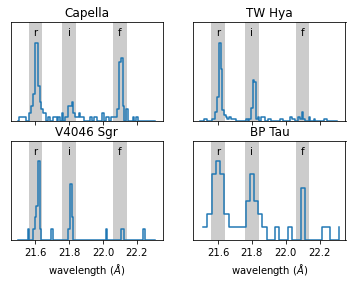
\includegraphics[width=0.49\textwidth]{figs/o7f2i.png}
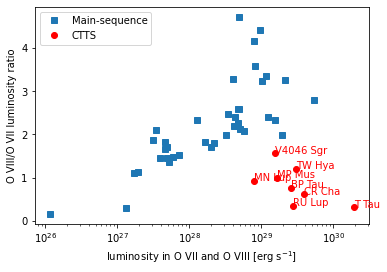
\includegraphics[width=0.49\textwidth]{figs/o72o8.png}
\caption{Signatures of accretion in classical T Tauri stars from high-resolution grating spectroscopy. \emph{Left:} Density-sensitive O~{\sc vii} triplet. Capella is a main-sequence star with an $f/i\sim 4$, while the other three sources are examples of CTTS with $f/i < 1$. All lines are unresolved, they appear wider in BP~Tau because the data is taken with a lower-resolution spectrograph (Chandra/LETG, while the other three are Chandra/HETG). \emph{Right:} Ratio of O~{\sc viii} to O~{\sc vii} line flux compared to the total flux in oxygen lines. All acrreting sources are well offset from the main-squence stars, indicating additional soft emission plasma. Modified from Ref.~ \cite{2013ApJ...771...70G} (see there for data sources) \label{fig:softexcess}}
\end{figure}

A related diagnostic is looking at the ratio of two ions of the same element. Figure~\ref{fig:softexcess} (right) shows the ratio of the flux in O~{\sc viii} to O~{\sc vii}. CTTS show lower O~{\sc viii}/O~{\sc vii} ratio than main-sequence stars of comparable luminosity, indicating CTTS emission is dominated by cooler plasma \cite{2007A&A...473..229R,2007A&A...474L..25G}. Looking from a different angle, one might also interpret this figure as  CTTS having a O~{\sc viii}/O~{\sc vii} much more in line line with low-luminosity main-sequence stars, and because there is a relation that brighter coronae are also hotter, this also leads to the conclusion that CTTS have additional cool plasma compared to normal corona. Again, this plasma can be interpreted as accretion-powered.

A third and more controversial observation is that CTTS usually show abundances that the Ne enhanced and Fe depleted compared to solar abundances. This pattern is seen in active stars, where it is attributed to element separation in the corona due to different values of the first ionization potential (FIP) of ions. Neon has a particularly high FIP and iron a particularly low one, so the pattern observed is called IFIP (inverse FIP). However, CTTS are cooler than main-sequence stars of comparable luminosity and so alternative scenarios have been discussed. Since accretion comes from the inner edge of the accretion disk, it is possible that disk process separate elements. If gain-forming elements condense into grains, pebbles, and proto-planets, the material on the inner disk edge might be depleted of Fe, Si, and similar metals, while noble gases stay in the gas phase and are thus preferentially accreted. \textcolor{blue}{HMG: This paragraph still needs some references.}

Early simulations of the accretion shock follow a 1D description of the flow. This approach is sufficient to match CCD-level resolution X-ray data. The accretion shock produces plasma matching the observed X-ray temperatures \citep{lamzin_1998} and the total energy in the accretion stream can be determined from fitting UV and optical spectra to determine the mass accretion rate \citep{calvet_1998}. Even early observations of the density-sensitive line ratios in He-like triplets such as in Fig~\ref{fig:softexcess} (left) can be explained by 1D models assuming a combination of accretion shock and coronal plasma \cite{Guenther_2007}. 

Before we discuss the shortcomings of the 1D approach and how more complex models can provide additional insight into the accretion shock structure, we want to present the fundamental physics that happens in accretion shocks. The following section assumes 1D for simplicity.


\subsection{Physics of accretion in 1D}
\label{sect:accretionphysics}

Accretion happens when mass from the circumstellar disk is transferred onto the stellar surface. In the basic model of magnetically funneled accretion, the stellar high-energy radiation ionizes the inner edge of the disk. When the stellar magnetic field connects to the inner edge of the disk, matter can flow along the field lines and impact onto the star, where a strong shock forms. The accretion column is relatively cool, but in the shock that gas is heated up to X-ray emitting temperatures. Depending on the exact location of the shock, those X-rays may or may not be visible, but the shock certainly heats the surrounding photosphere, which causes bright UV emission and an optical veiling (a strong continuum that makes phtotospheric emission lines appear weaker than in a non-accretion star.)

As the star and the disk rotate, and the magnetic field and the disk structure evolves, the accretion geometry and the accretion rate can change on time scales as short as minutes or as long as centuries; accretion can also switch off temporarily or permanently, as the star looses its disk. Despite that, many basic aspects of the accretion physics can be described in a 1D model where all mass motion happens parallel to the magnetic field. In the next few sub-sections we review some of the basic physics of accretion columns and accretion shocks. While modern models go far beyond such a simple prescription, the foundation of all accretion shock models still is to convert the graviational energy in the disk to kinetic energy of the infalling gas, which in turn gets turned into heat and radiation in the accretion shock.

\subsubsection{Free-fall velocity}
The free fall velocity $v_{\textnormal{free}}$ of material coming from an inner disk radius of $R_\mathrm{in}$ onto a star with mass $M_*$ and radius $R_*$ is
\begin{equation} 
v_{\textnormal{free}} = \sqrt{{2GM_*} \left(\frac{1}{R_*} - \frac{1}{R_\mathrm{in}}\right)} \approx 620 \sqrt{\frac{M_*}{M_\odot}}\sqrt{\frac{R_\odot}{R_*}} \frac{\textnormal{km}}{\textnormal{s}}\ \label{eqn:freefall} 
\end{equation}
where $G$ is the gravitational constant. The inner radius is typically a few stellar radii and thus $v_\textnormal{ff}$ is very close to infall from infinity.


\subsection{Calculation of shock front}
All turbulent fluxes are neglected and we only treat stationary shocks. In the shock front, ions and electrons are heated differently, but they remain strongly coupled and reach the same temperatures with in a few mean-free path lengths - a region so thin that it is justified to treat them as a single fluid. 

Somewhere along the accretion column, a shock forms when the forward ram pressure becomes comparable to the pressure of the underlying material. The shock front itself is very thin, only of the order of a few mean free paths \cite{raizerzeldovich}. Therefore it can be treated as a mathematical discontinuity described by the Rankine-Hugoniot jump-conditions \cite[][chap.~7, \S~15]{raizerzeldovich}; in the shock the super-sonic infall velocity is converted mostly into thermal energy. To simplify the numerical treatment we assume the direction of flow parallel to the magnetic field, so the Lorentz force does not influence the dynamics. Marking the state in front of the shock front by the index 0, that behind the shock by index 1, the Rankine-Hugoniot conditions become
\begin{eqnarray}
\rho_0 v_0 &=& \rho_1 v_1 \label{RH1}\\
P_0+\rho_0 v_0^2 &=& P_1+\rho_1 v_1^2 \label{RH2}\\
\frac{5 P_0}{2\rho_0}+\frac{v_0^2}{2}&=&\frac{5 P_1}{2\rho_1}+\frac{v_1^2}{2} \ ,\label{RH3}
\end{eqnarray}
where $v$ is the velocity, $\rho$ the total mass density of the gas and $P$ its pressure. 

From the jump conditions, the shocks will heat gas to a temperature
\begin{equation}
kT \simeq \frac{3}{16}\mu m_p v^{2} \approx 0.3\,{\rm keV}\left(\frac{v}{500\,{\rm km/s}}\right)^{2} \approx3.5\times10^6\,{\rm K} \left(\frac{v}{500\,{\rm km/s}}\right)^{2},
\label{eqn:Tshock}
\end{equation}
where $\mu$ is the dimensionless atomic weight.

\subsubsection{Structure of the post-shock region}

In the following section we compute how the originally different kinetic temperatures of ions and electrons as well as the ionisation temperature
equilibrate and calculate the emitted X-ray spectrum.

\paragraph{Momentum balance}\label{hydrodyn}

In the post-shock region the gas emits radiation and cools down, so the energy of the gas is no longer conserved.  However, the particle number flux $j$ of ions (and atoms) 
\begin{equation}j=nv\label{j_n}\end{equation}
is conserved, where $n$ is the ion/atom number density; the electron number density is denoted by $n_{\mathrm{e}}$. The total momentum flux $j_p$ is conserved, since we ignore the momentum loss by radiation; it consists of the ion and the electron momentum as follows:
\begin{eqnarray}  
j_p&=&\mu m_{\mathrm{H}} n v^2+P \nonumber \\
   &=&\mu m_{\mathrm{H}} n v^2+nkT \label{j_p}
\end{eqnarray}
with $P$ is the thermodynamic pressure and $T$ the temperature; $m_{\mathrm{H}}$ denotes the mass of a hydrogen atom.

\paragraph{Energy balance}
\label{sect:energybalance}

Let us next consider the energy balance in the post-shock region. In general,  
\begin{equation} \label{tsminuspdvisdu} T d\Sigma -P dV=dU \end{equation}
where $\Sigma$ denotes the entropy and $U$ the internal energy of the plasma. The quantity $T d\Sigma=dQ$ denotes the heat flux through the boundaries of the system; one important component of the is the energy loss $Q_{col}$ through collisions that excite higher electronic states, which will than decay through radiation. 

Assuming that the shock location is stationary, we get $\frac{d}{dt}=\frac{\partial}{\partial t}+\frac{\partial z}{\partial t}\frac{\partial}{\partial z}=v\frac{\partial}{\partial z}$ depending on the location $z$, measured from the shock front inwards; differentiation with respect to $z$ will be indicated by $'$.
The internal energy $U$ is in this case the thermal energy $U=\frac{3}{2}kT$, the pressure $P$ can be rewritten using the equation of state. The specific volume $V$ is the inverse of the number density $V=\frac{1}{n}$. 
It is convenient to write the electron number density as \mbox{$n_{\mathrm{e}}=x_e n$,} with $x_e$ denoting the number of electrons per heavy particle.
\begin{equation}
\label{energyelec}
v\left(\frac{3}{2}x_e k T_{\mathrm{e}}\right)'+v x_e n k T_{\mathrm{e}} \left(\frac{1}{n}\right)'=-Q_{col} x_e n,
\end{equation} 

We now have $n$, $v$, and $T$ as variables and three hydrodynamic equations (\ref{j_n}, \ref{j_p}, and \ref{energyelec}), so the structure of the post-shock region can be calculated.


\subsection{Observed shortcomings of stationary 1D models}
While 1D models are successful in many aspects, there are observational and theoretical arguments that important physical processes are not captured in 1D. In deep Chandra observations of TW~Hya, densities can be measured in three density-sensitive triplets. The density is highest in Mg~{\sc xi} and lowest in O~{\sc vii}, although Mg~{\sc xi} is formed at a higher temperature \cite{Brickhouse_2010}. Thus, one would expect Mg~{\sc xi} emission from a region directly behind the accretion shock and O~{\sc vii} from denser layers deeper down. One possible explanation is that the observed O~{\sc vii} emission is not from the accretion shock itself, but originates in hot material that escapes the accretion column to the side and is denser than a normal stellar corona, but not as dense as plasma behind the accretion shock. That in turn means that the total X-ray flux might not be a good measure of the total accretion rate. 

This is corroborated by the surprising observation that X-ray determined mass accretion rates are very similar for most sources despite a difference in optically determined mass accretion rate by three orders of magnitude \cite{2011A&A...526A.104C} which can be explained if the accretion streams are not homogeneous structures but have a density profile and the inner layers either form shocks deeper in the atmosphere or simply have they X-ray emission reprocessed by the outer layers of the accretion stream \cite{2018A&A...618A..55S,2021Natur.597...41E}.

Time variability can give us another insight. In V4046~Sgr the emission lines from soft, presumably shocked, plasma have a period of exactly have the orbital period of the close binary. Together with Doppler-imaging this leads to the interpretation that we can observe the shock only when the accretion flow is perpendicular to the line of sight, while the accretion funnel blocks the view of the shocked region at other times \cite{2012ApJ...752..100A}. Similarly, the accretion funnel has been observed to block the X-rays from AA~Tau for certain rotational phases. This includes coronal and accretion generated X-rays \cite{2007A&A...462L..41S,2007A&A...475..607G}. 
There are several other classes of time-variable pre-main sequence accretors, including FU~Ors and EX~Ors, where the accretion rate changes by orders of magnitude or stars where a change in the disk structure moves absorbing material into our light of sight, such as in RW~Aur or also in AA~Tau. However, those changes happen on much larger scales than the accretion shock itself and are not discussed here any further.

Similarly, improved models including LTE radiation transfer now show that the heated photosphere does not radiate as a simple black body in the optical and infrared \cite{Dodin_2012,Dodin_2013}, but that is also produces lines, which selectively fill in some photospheric absorption lines, possibly biasing accretion rate measurements based on optical veiling.



\begin{figure}
    \centering
    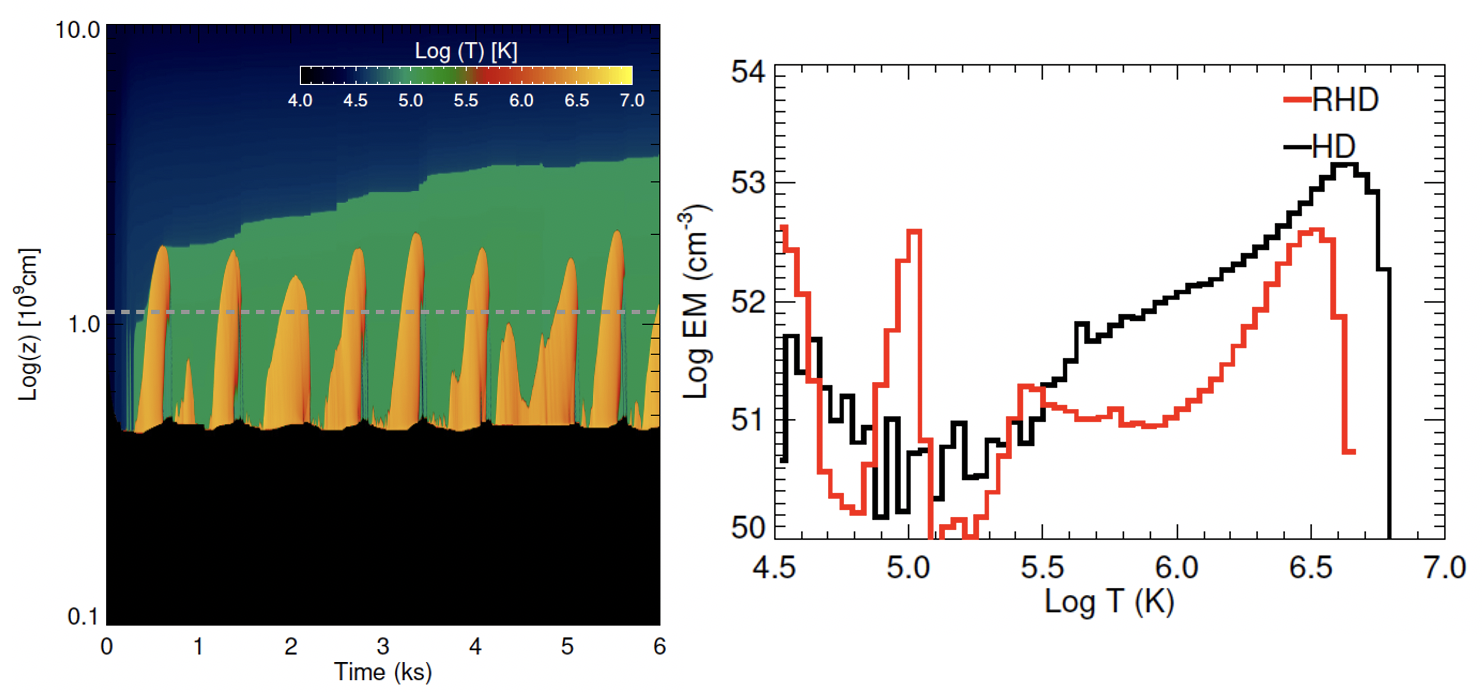
\includegraphics[width=11cm]{figs/colombo2019b.png}
    \caption{A combination of Fig. 3 and Fig. 5 from Colombo et al. 2019b. As far as I know the only non-LTE simulation of the accretion region. Need from permission. I would select one of the figures, Colombo 2016 or Colombo 2019b.}
    \label{fig:colombo2016}
\end{figure}

\begin{figure}
    \centering
    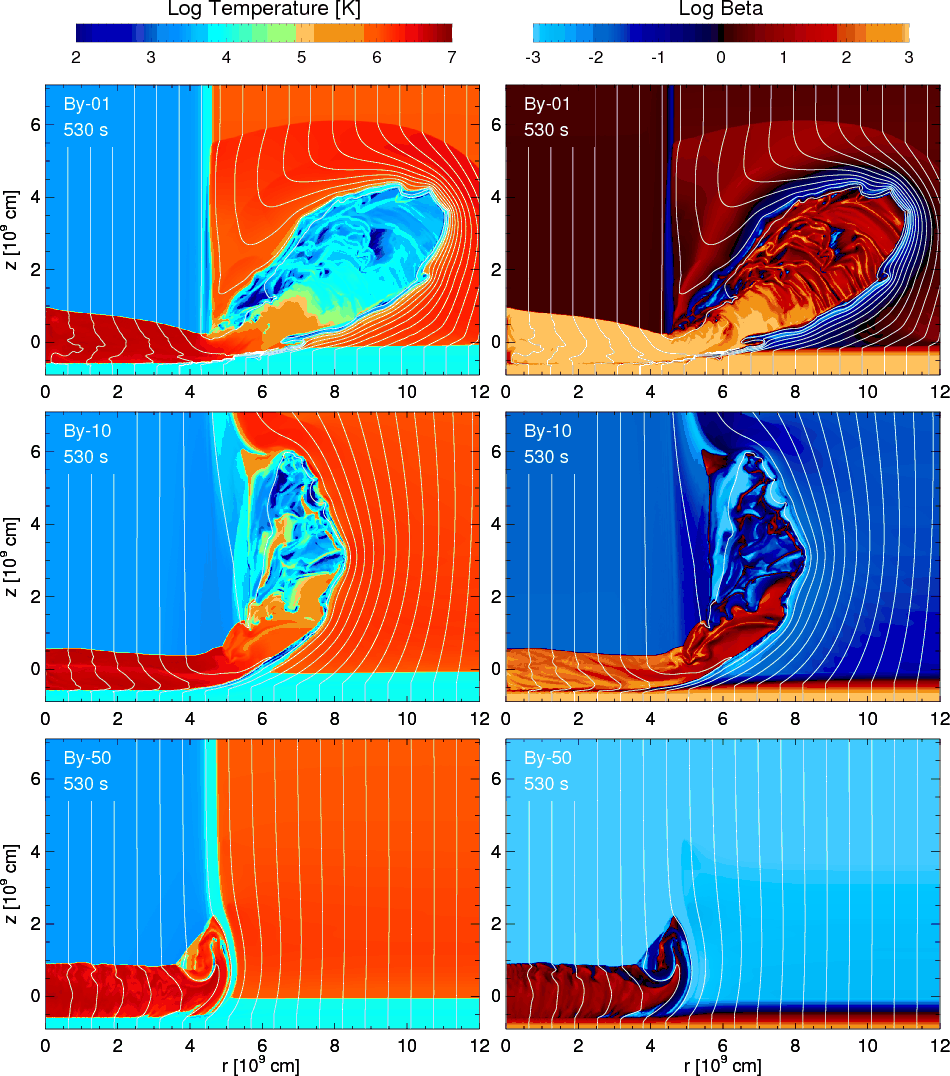
\includegraphics[width=11cm]{figs/Sacco2010.png}
    \caption{Moritz: I've always liked this figure. It's over a decade old at this point but it has the "spill-out" on the side that observers often have in mind and I think it's easier to interpret than a figure with time on the x-axis. Or is this so out of date that it's simply not OK to use that any longer? THe REvet et al 2017 would work for the same purpose. I would select one of the figures, Colombo 2016 or Colombo 2019b or this one.}
    \label{fig:sacco2016}
\end{figure}

\textcolor{blue}{
- When we start to talk about numerical models we should introduce MHD equations. Transition from analytical to numerical models in this subsection?}

\textcolor{blue}{- I would not call the models above this section "analytical". Lamzin 2004, Calvet \& Gulbring and my own Guenther 2007 are all numerical models solving HD equations - admittedly in 1D, but including radiative losses, so it's a numerical, not an analytic solution. So, in my mind, the questions is if we transition from 1D HD (some of those models might be 1D MHD, but if the B field is parallel to the one model dimension you have, that's essentially HD) to 3D MHD and this might be a good place to do that.}

\subsection{The multi-D structure of the accretion shock}

Most observations of the structure of the accretion shock on young stars are spatially unresolved; only Doppler-imaging can at least reveal the location on the surface where the accretion shock happen. Yet, it would be very valuable to learn about the detailed 3D geometry and the time evolution of accretion shocks to interpret the unresolved data. For example, it is unclear if the accretion shocks forms deeply in the photosphere where it is hidden from view or higher up in the accretion funnel. One approach to address this problem is to perform experiments in the laboratory using a set-up where magnetic fields, densities, temperatures, and other hydrodynamical parameters are chosen to scale to the stellar case. Such work finds that plasma is ejected laterally from the accretion shock and forms a shell around the infalling stream \cite{2017SciA....3E0982R} . This hot shell provides an additional absorber that reduces the shock emission that is directly observable. Recently, new laboratory experiments tested accretion streams not perpendicular to the impacted surface as it might happen for accretion stream along complex magnetic field structures. They find the resulting plasma flows to be highly asymmetric and see a large amount of plasma escaping laterally from the accretion flow \cite{2020A&A...642A..38B}.  

Another approach is to look for analogous situations in our Sun, where spatially resolved data in the UV and EUV, even if not in X-rays, is available with long time coverage and high cadence. One particular event happened on June, 7$^{th}$, 2011, when parts of an erupting filament fell back into the Sun \cite{2013Sci...341..251R,2013A&A...559A.127O}. The infall speed of up to 450~km/s was comparable to free-fall accretion onto T Tauri stars, but the accretion rate was obviously much lower. Similar to the laboratory experiments, the initial infall triggered upflows, but here they shocked with later fragments causing UV emission.

Both, laboratory experiments and the solar analogy, point to a significantly more complex picture than the simple 1D accretion shock outlined above. Simulations of the accretion shock \textcolor{blue}{Sabrina, do you want to conitnue here? Structure of the accretion shock in X-rays: Orlando, Bonito, Colombo; figure?}

\begin{figure}
    \centering
    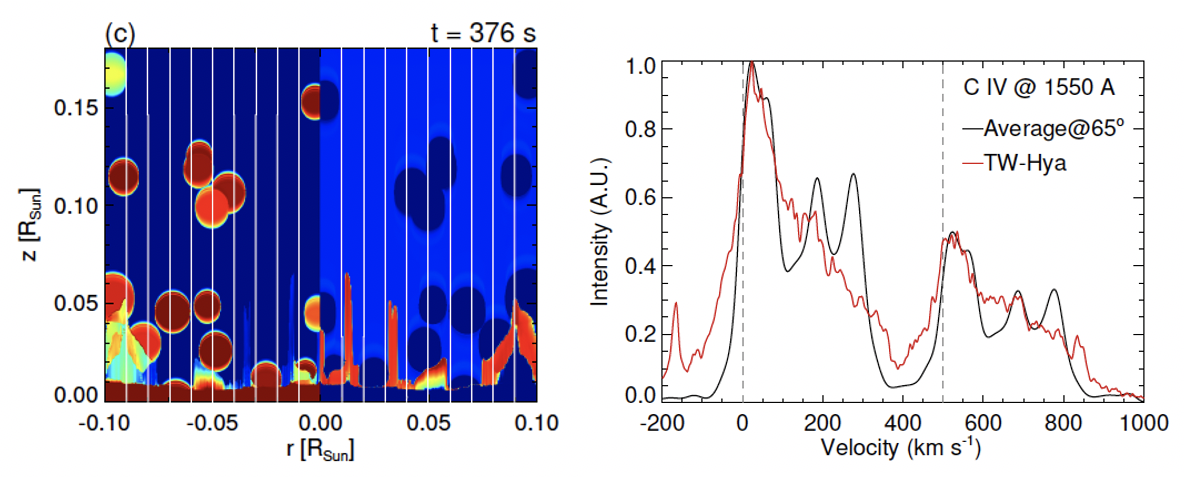
\includegraphics[width=11cm]{figs/colombo2016.png}
    \caption{A combination of Fig. 3 and Fig. 6 from Colombo et al. 2016. Interesting for the fragmented structure of the accretion stream which reproduces the CIV profiles (X-rays and other observations). Need for permission. I would select one of the figures, Colombo 2016 or Colombo 2019b.}
    \label{fig:colombo2016}
\end{figure}

\begin{figure}
    \centering
    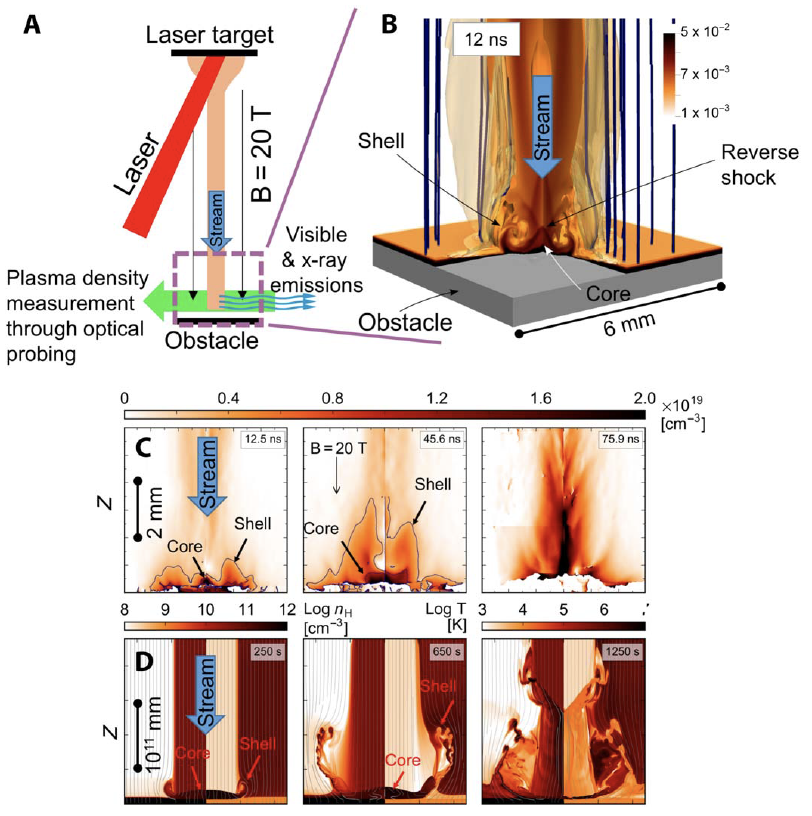
\includegraphics[width=11cm]{figs/Revet2017.png}
    \caption{Another possibility from Revet et al. 2017. Here they combine laboratory experiments with MHD simulations. Need to ask for permission.}
    \label{fig:revet2017}
\end{figure}



\section{Jets}
 {\color{blue}        (10 pages)}


\begin{figure}[t]
 \centering
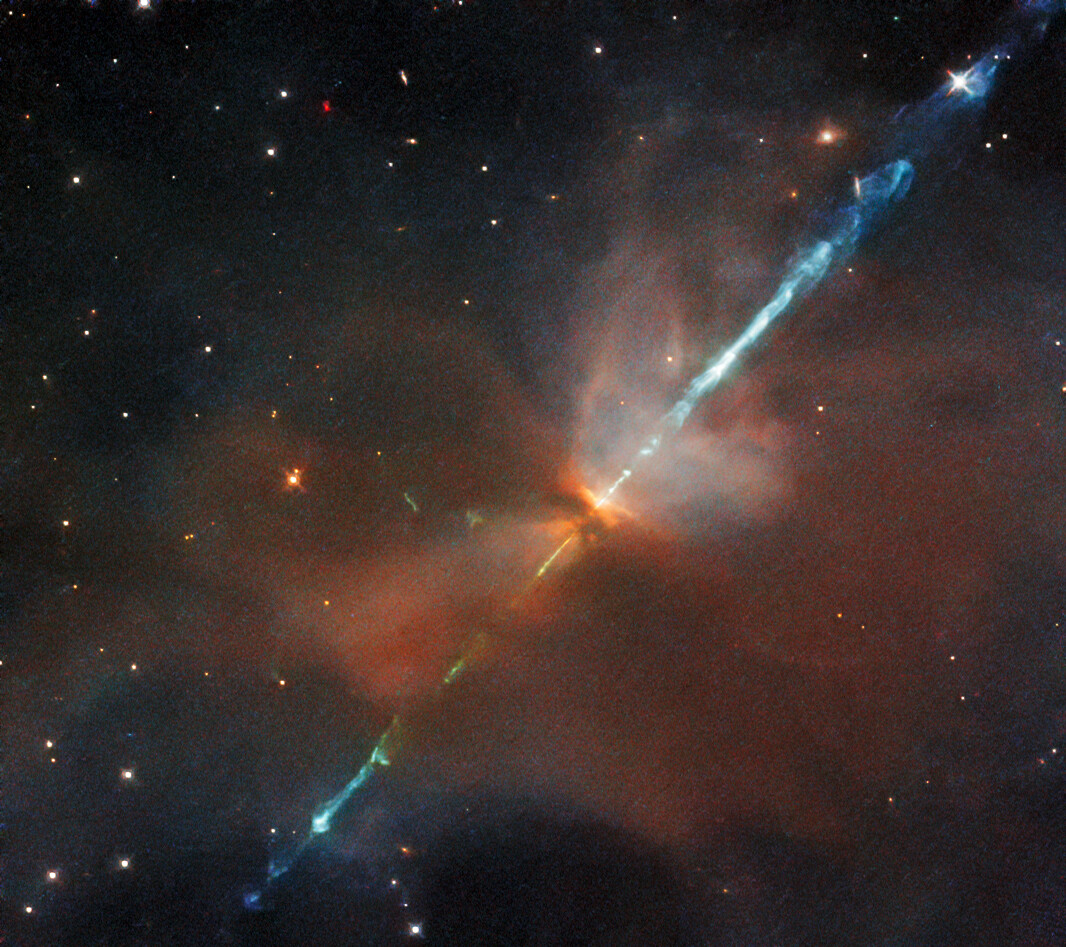
\includegraphics[width=6cm]{figs/HH111_-_HST_-_Potw2135a.jpg}
\caption{HST composite image of HH~111. Image credit: ESA/Hubble \& NASA, B. Nisini. \label{fig:HH111} }
\end{figure}


% https://en.wikipedia.org/wiki/File:HH111_-_HST_-_Potw2135a.jpg

A variety of mass ejection phenomena occur during the first stages of star evolution which are intimately related to the accretion process described in the previous section. In general, plasma is ejected from a young stellar system, which then propagates in the ambient medium with supersonic velocities. Outflows in pre-main sequence stars (PMS) are detected in a wide range of wavelengths and show very different morphologies, from jets to less-collimated, wide-angle outflows. In this section, we focus on protostellar jets which are well collimated beams (opening angles of a few degree)

Most jet observations are compatible with MHD winds launched from the inner regions of protoplanetary disks \citep{Frank_2014}. However, there are other possible launch regions. First, stellar winds launched from the hot stellar corona much like the solar wind \citep{Matt_2005}. In analogy with the solar wind, such stellar winds are very hot ($\gtrsim10^6$\,K) and may cool via X-ray emission. Second, magnetospheric ejections launched from the region between the star and the inner edge of the disk \citep{Zanni_2013}. Third, X-winds are launched from a narrow region close to the inner edge of the disk \citep{Shu_1994}. Even more mechanisms to launch outflows may exist  in the young, class~0 objects, but they produce slower outflow velocities and are therefore related to the observed X-ray emission and ignored here.

{\color{red} TBD: Magnetic towers \citep{Huarte_2012}? }

Observationally,  protostellar outflows  were ``discovered''\footnote{The nebulosity around T~Tau was first described in the 19th century  by \citet{Burnham_1890, Burnham_1894}.} by \citet{Herbig_1950,Herbig_1951} and \citet{Haro_1952,Haro_1953}. These authors studied the optical, nebular emission, mostly from forbidden emission lines (FELs), which is typically concentrated in individual, relatively distinct emission regions along the jet path and these so-called knots or chains of knots are called Herbig-Haro (HH) objects (see Fig.~\ref{fig:HH111} for a beautiful example). Protostellar jets are bright in FELs, because shocks within the outflow heat the outflowing plasma to temperatures of roughly $10^4\,$K \citep{}. According to Eq.~\ref{eqn:Tshock}, such a post shock temperature corresponds to shock velocities of $\sim20-30$\,km\,s$^{-1}$.
%
Because of the low densities ($\lesssim10^4\,$cm$^{-3}$ beyond few tens of au), radiative cooling of the shock heated plasma is dominated by hydrogen (e.g., H$\alpha$) and metalic forbidden emission lines like [O~{\sc i}], [S~{\sc ii}], and [Fe~{\sc ii}]. These lines (or line ratios) allow one to estimate the physical properties of the emitting plasma \citep[temperature, density, ionization degree, e.g., ][]{Bacciotti_1999}.

Since their discovery, protostellar jets were studied in a variety of wavelengths, from radio \citep{} to (near-) IR \citep{}. However, there were simply no indications for plasma temperatures well in excess of several tens of thousands of K; emission from [O~{\sc iii}] were considered ``high-ioniziation'' in the protostellar jet context. Hence, the detection of protostellar jets in X-rays came to a surprise.

\subsection{X-rays from protostellar jets}


%
% \begin{figure}[t]
% \centering
%
% 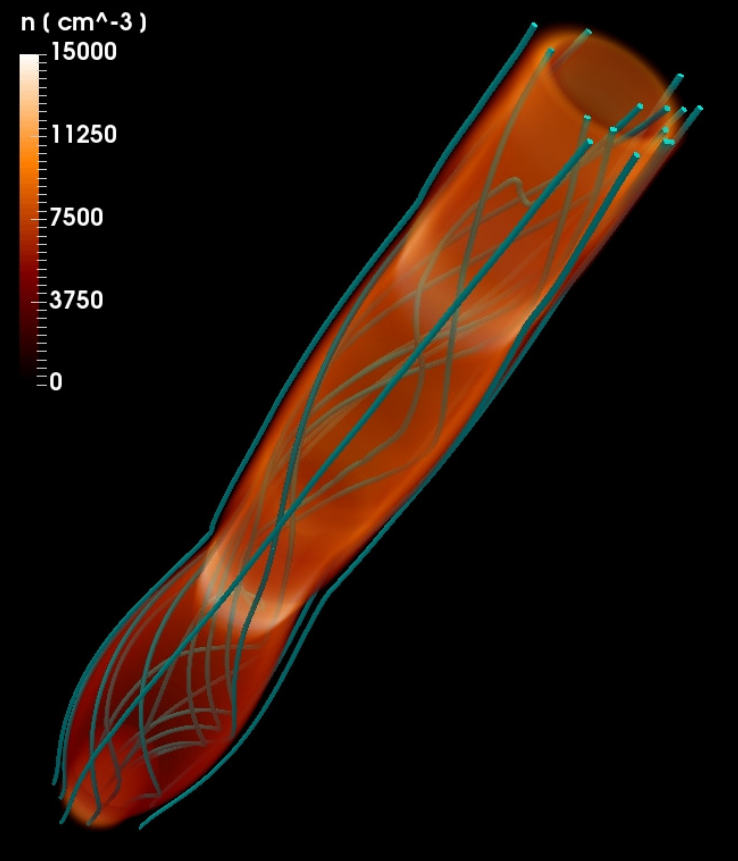
\includegraphics[height=6cm]{figs/diamond}
% % % %
% %  \vspace*{-0.5cm}
%  %
%  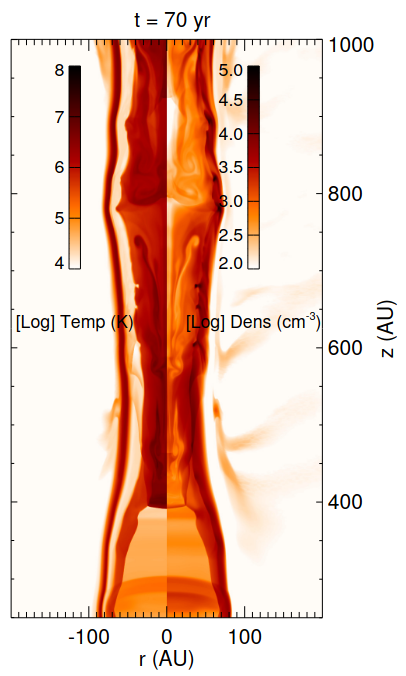
\includegraphics[height=7cm]{figs/diamond_simu}
%
% \caption{{\bf Left: } Structure of jet and magnetic field close to the base. From \citet{Ustamujic_2016}.
%          {\bf Right: }. From \citet{Ustamujic_2018}. \label{fig:jet_simu}}
% \end{figure}




\begin{figure}[t]
\centering

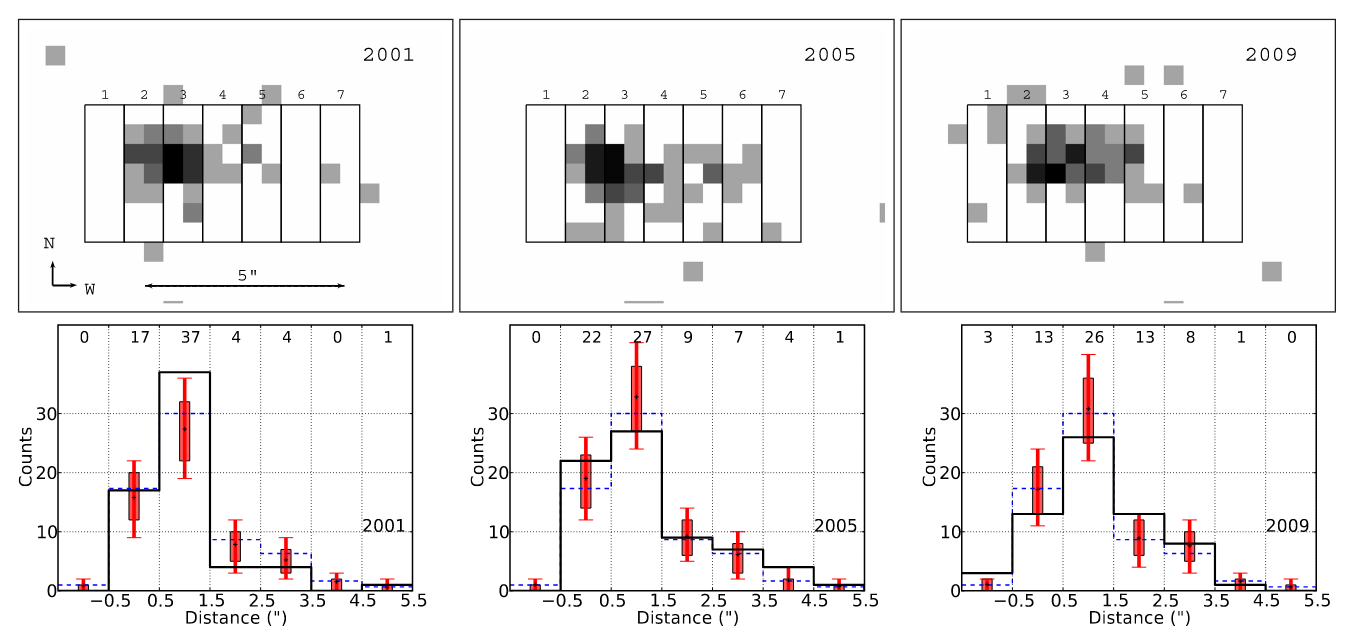
\includegraphics[height=6cm]{figs/hh154}
% % %
\caption{Evolution of the X-ray emission from HH 154. From \citet{Schneider_2011}. \label{fig:hh154}}
\end{figure}


% \subsection{X-ray jet observations}
The first X-ray detections of protostellar jets were obtained almost simultaneously in 2001 by \citet{Pravdo_2001} using Chandra (HH~2) and \citet{Favata_2002}
using XMM-Newton (HH~154 or L~1551~IRS\,5). Both HH objects are launched from class~I objects. The association of the Chandra detected X-ray emission to HH~2 straight forward, because the X-ray emission  (a) spatially coincides with one of the optically brightest knots within HH~2, (b) appears extended, and (c) the spectrum is soft ($T\sim1.2\times10^6\,$K) unlike typical coronae of young stars. In contrast, the association of the X-rays from the L\,1551~IRS\,5 complex to HH~154 strongly builds on the severe extinction towards the protostellar sources while the jet suffers much less extinction \citep[$A_V(jet)\sim10\,$mag vs $A_V(protostars)\gtrsim150$\,mag, e.g.,][]{White_2000,Fridlund_2005}. This high $A_V$ towards the stellar sources led \citet{Favata_2002} to ascribe the X-rays to HH~154 despite the proximity of the X-ray emission with the stellar position and the comparably high mean X-ray energies ($\sim1\,$keV), simply because any reasonable X-ray emission from the stellar system would not make it directly to the observer. Later, \citet{Bally_2003} located the X-rays from HH~154 to the base of the outflow using new Chandra data but also find a higher temperature for the emitting plasma and, thus, reconsider the origin of the X-rays discussing reflection of stellar X-rays from one (or a combination) of the protostars by some medium close to the stars and a variety of shocks, e.g., within the outflow, against one disk, or between the stellar winds of the individual protostars of the system. These authors already note that the location of the X-rays may be in a region where the outflow is collimated to the narrow jet observed further away from the sources, which turned out to be, at least obserationally, a relatively common feature and the X-ray emission of protostellar jets can be broadly divided into emission from the jet base and from working surfaces at large distances to the driving sources.

X-ray emission close to the base of the jet, and far away (HH objects) also due to interaction with dense CSM or molecular clouds.



\subsubsection{X-rays from the jet base}




\begin{figure}
    \centering
    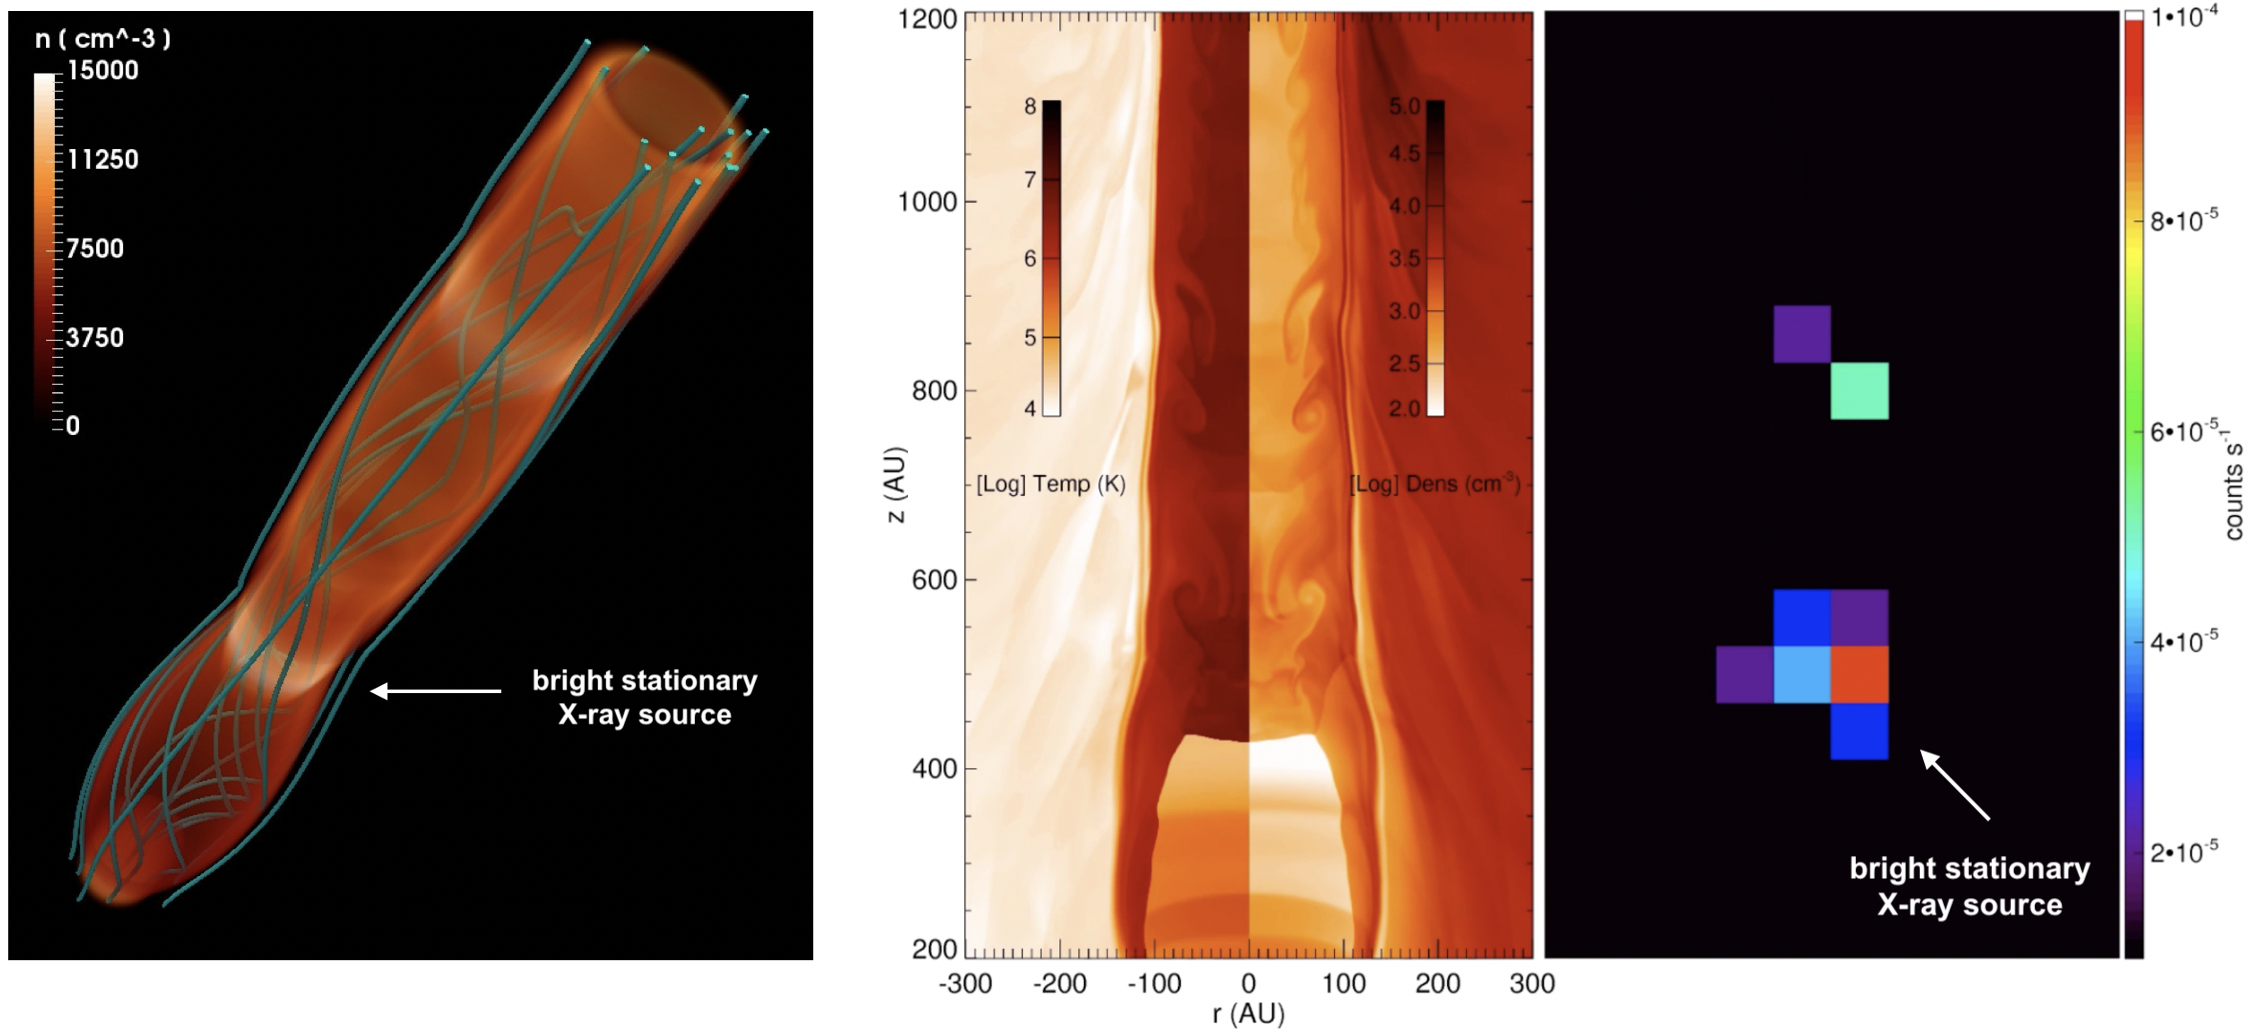
\includegraphics[width=12cm]{figs/ustamujic.png}
    \caption{A combination of Figs. from Ustamujic et al. 2016,2018,2019. I'd rather prefer this one in order to include the X-ray emission synthesized from the model (which is in agreement with the observations).}
    \label{fig:ustamujic}
\end{figure}



\begin{figure}[t]
% \centering

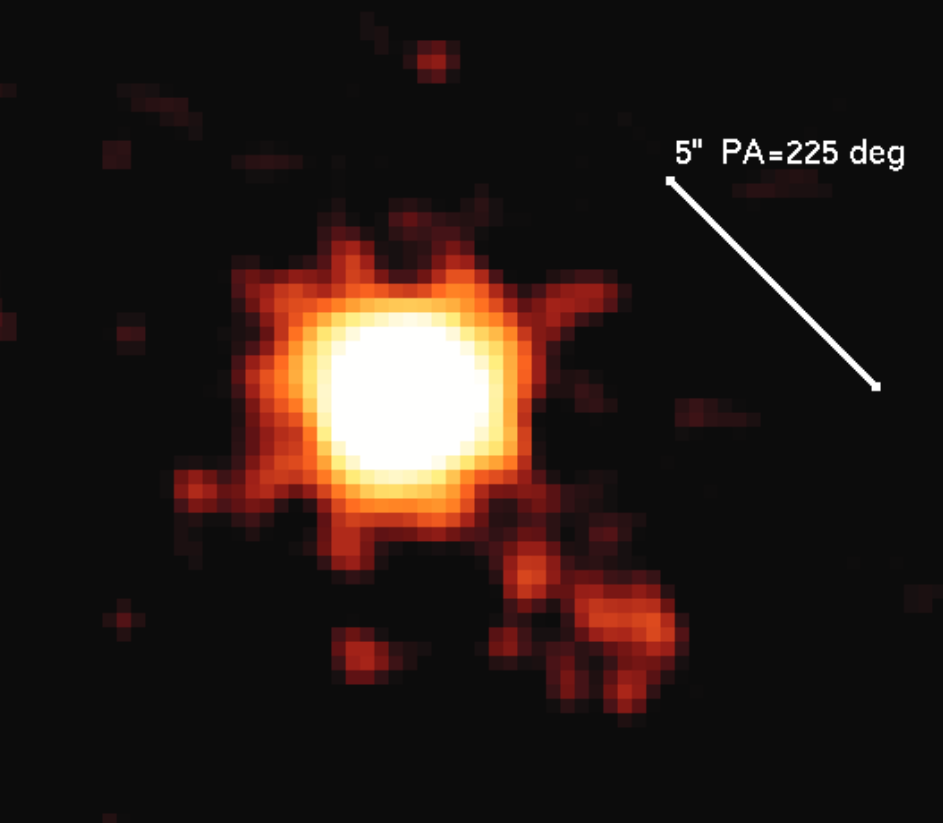
\includegraphics[width=6cm]{figs/dg_tau_X}
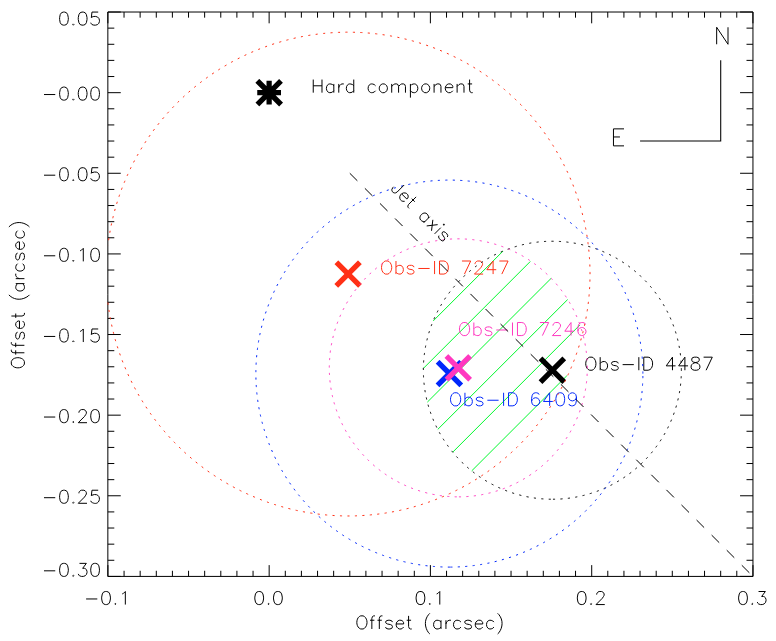
\includegraphics[width=6cm]{figs/dg_tau_offsets}

\caption{{\bf Left: } Chandra X-ray image of the DG~Tau system. From \citet{2011ASPC..448..617G}.
         {\bf Right: } Relative spatial offsets between the hard (coronal) and soft (jet) emission. From \citet{Schneider_2008}. \label{fig:dg_tau_X}}
\end{figure}


\subsubsection{X-rays from jet knots}

{\color{blue}(jet origin, collimation, jet velocities) [Christian, Sabina]}


Sketch (suggestion?) should we make a new sketch? Is Fig.~\ref{fig:jet_simu} left sufficient?
I think that it's sufficient. If we have enough space I would separate the panels in two figures: left panel to talk about the physics and the right one for the X-ray emission from jets.

Wind, outflows and jets: Bally 2016 (main components of outflows); Matt \& Pudritz 2005 (accretion powered winds), Zanni \& Ferreira 2013 (magnetospheric ejections)

Jet origin, ejection and collimation here.
MHD model magnetospheric ejections Zanni \& Ferreira 2013

\begin{figure}
    \centering
    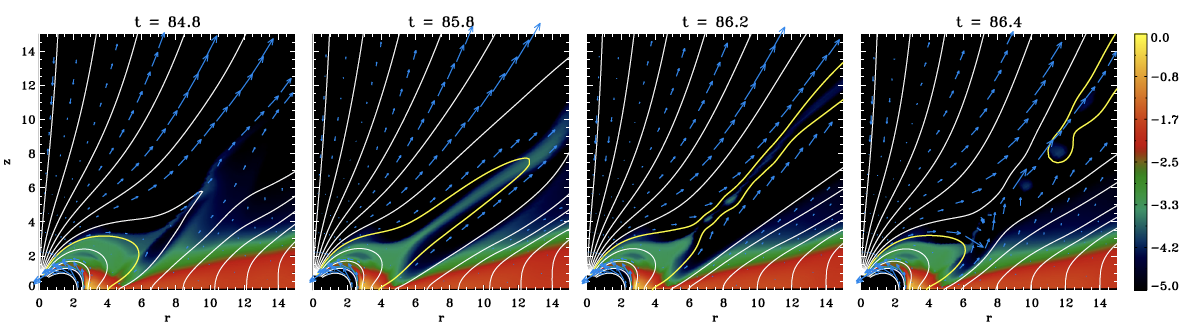
\includegraphics[width=12cm]{figs/Zanni2013.png}
    \caption{Temporal evolution of the periodic inflation/reconnection process which characterizes the dynamics of the magnetospheric ejections. Need to ask for permission.}
    \label{fig:zanni2013}
\end{figure}

{\color{blue}Christian

Favata HH 154, Guedel DG Tau, Schneider HH 154

Laboratory experiments  e.g. Revet et al. 2017
}

X-ray discovered jets: HH 2 \citep{Pravdo_2001,Schneider_2012}, HH 154 \citep{Favata_2002,Bally_2003,Favata_2006,Schneider_2011}, HH 168 \citep{Pravdo_2005,Schneider_2009}, DG Tau \citep{Guedel_2005,Guedel_2008,Schneider_2008}, Z CMa \citep{Stelzer_2009}, RY Lup \citep{Skinner_2011}, HD~163296 \citep{Swartz_2005,Guenther_2013}, TAX \citep{Guedel_2007}, HH~80/81 \citep{Pravdo_2004}, HH~210 \citep{Grosso_2006}, HH~248 \citep{Lopez_2015}.

\subsection{Models of jets}

A paragraph about models to study the launching site.

Different scales

\subsubsection{Modelling of X-ray emitting jets}
\citet{Raga_2002}

HD models (Bonito), MHD (Ustamujic) and comparison with observations

X-ray emitting close to the base
Far away

\subsubsection{Mass loss rate}

\subsection{Plasma cooling \label{sect:cooling}}
Three processes contribute to the cooling of a plasma: Radiative cooling, cooling by expansion and thermal conduction.
The pressure work done by the plasma is $\delta W = p dV$ and the radiative losses are
\begin{equation}
\delta Q_{rad} = -n_e^2 V(t) \Lambda(T) dt\,,
\end{equation}
where $n_e$ is the electron density, $V$ the volume and $\Lambda(T)$ is the cooling function.
The conductive heat flux is given by
\begin{equation}
q_{cond} = -\kappa(T)\bigtriangledown T\,, \label{eq:cond}
\end{equation}
where the thermal conductivity according to Spitzer is
\begin{equation}
\kappa(T) = \kappa_0 \frac{T^{5/2}}{\ln \Lambda}\;\mbox{erg}\,\mbox{s}^{-1}\,\mbox{K}^{-1}\,\mbox{cm}
\end{equation}
with $\kappa_0=1.8\times10^{-5}$ and the Coulomb logarithm $\ln \Lambda$, which describes the collision properties of the plasma and is of order 10.
When the mean free path length for energy exchange is of the same order as the thermal scale height, the conduction should be approximated by the saturated flux
\begin{equation}
q_{sat} = 5 \phi \rho c_s^3\,,
\end{equation}
with $\phi\approx0.3$ \citep[e.g.][$\rho$ is the mass density and $c_s$ is the local sound speed]{Borkowski_1989}. For an estimate of the importance of the saturated flux, we assumed a linear temperature decrease. Under these circumstances the Spitzer value  exceeds the saturated flux on spatial scales of about 10\,AU for the cooling from $T_1=10^6$~K to $T_0=10^4$~K, i.e., the saturated flux should be used for these steep gradients ($n\approx10^3$).



Thermodynamics states that the energy change of a plasma cell is described by
\begin{equation}
dU + \delta W = \delta Q = \delta Q_{rad} + q_{cond}\cdot A\;dt\; \label{eq:cooling1}
\end{equation}
with the internal energy $U=\alpha N kT$ ($\alpha=3/2$ for a fully ionized plasma), the particle number $N$, the Boltzmann constant $k$, the temperature $T$  and $A$ is the surface area through which heat conduction proceeds.
We use $p=2n_ekT$ in the expression for the pressure work and follow \citet{Guedel_2008} by writing  eq.~\ref{eq:cooling1} as
\begin{equation}
\alpha \frac{dT}{T(t)} + \frac{dV}{V} = - \left( \frac{n_e \Lambda(T)}{2 k T(t)}+ \frac{\kappa_0}{2n_eVkT}\cdot A\frac{T^{5/2}}{\ln \Lambda} \nabla T \right) dt \,,\label{eq:cool}
\end{equation}
where we used $N_e=n_e\cdot V$ and note that this expression holds only in the presence of sufficiently small temperature gradients.


In order to estimate the relative importance of the three cooling terms, additional information is needed, in particular, the opening angle of the X-ray emitting jet, its density structure, the temperature gradient, the surface for the heat conduction, which would include the magnetic topology and the properties of the environment, e.g., its ionization. These quantities are not available for the X-ray emitting part of the jet. We therefore decided to give some order of magnitude estimates for the cooling times of the individual processes ignoring contributions of the other ones. As we will see, there are distinct regions in the parameter space where each process seems ApJ...576L.149Rto dominate, so we regard this approach reasonable.

Figure~\ref{fig:cooling} shows the cooling curves for the different processes assuming different parameters for the jet. For radiative and conductive cooling, the mapping of time to distance in this figure depends on the actual, deprojected space velocity of the plasma.
A rough estimate is 0.3\arcsec{}~yr$^{-1}$, which implies that today's inner X-ray emission will reach the position of today's outer emission in 15 years.
Adiabatic cooling, on the other hand, does not depend of the outflow velocity but only on the initial cross-section of the plasma and on the opening angle.


\begin{figure}
  \centering
   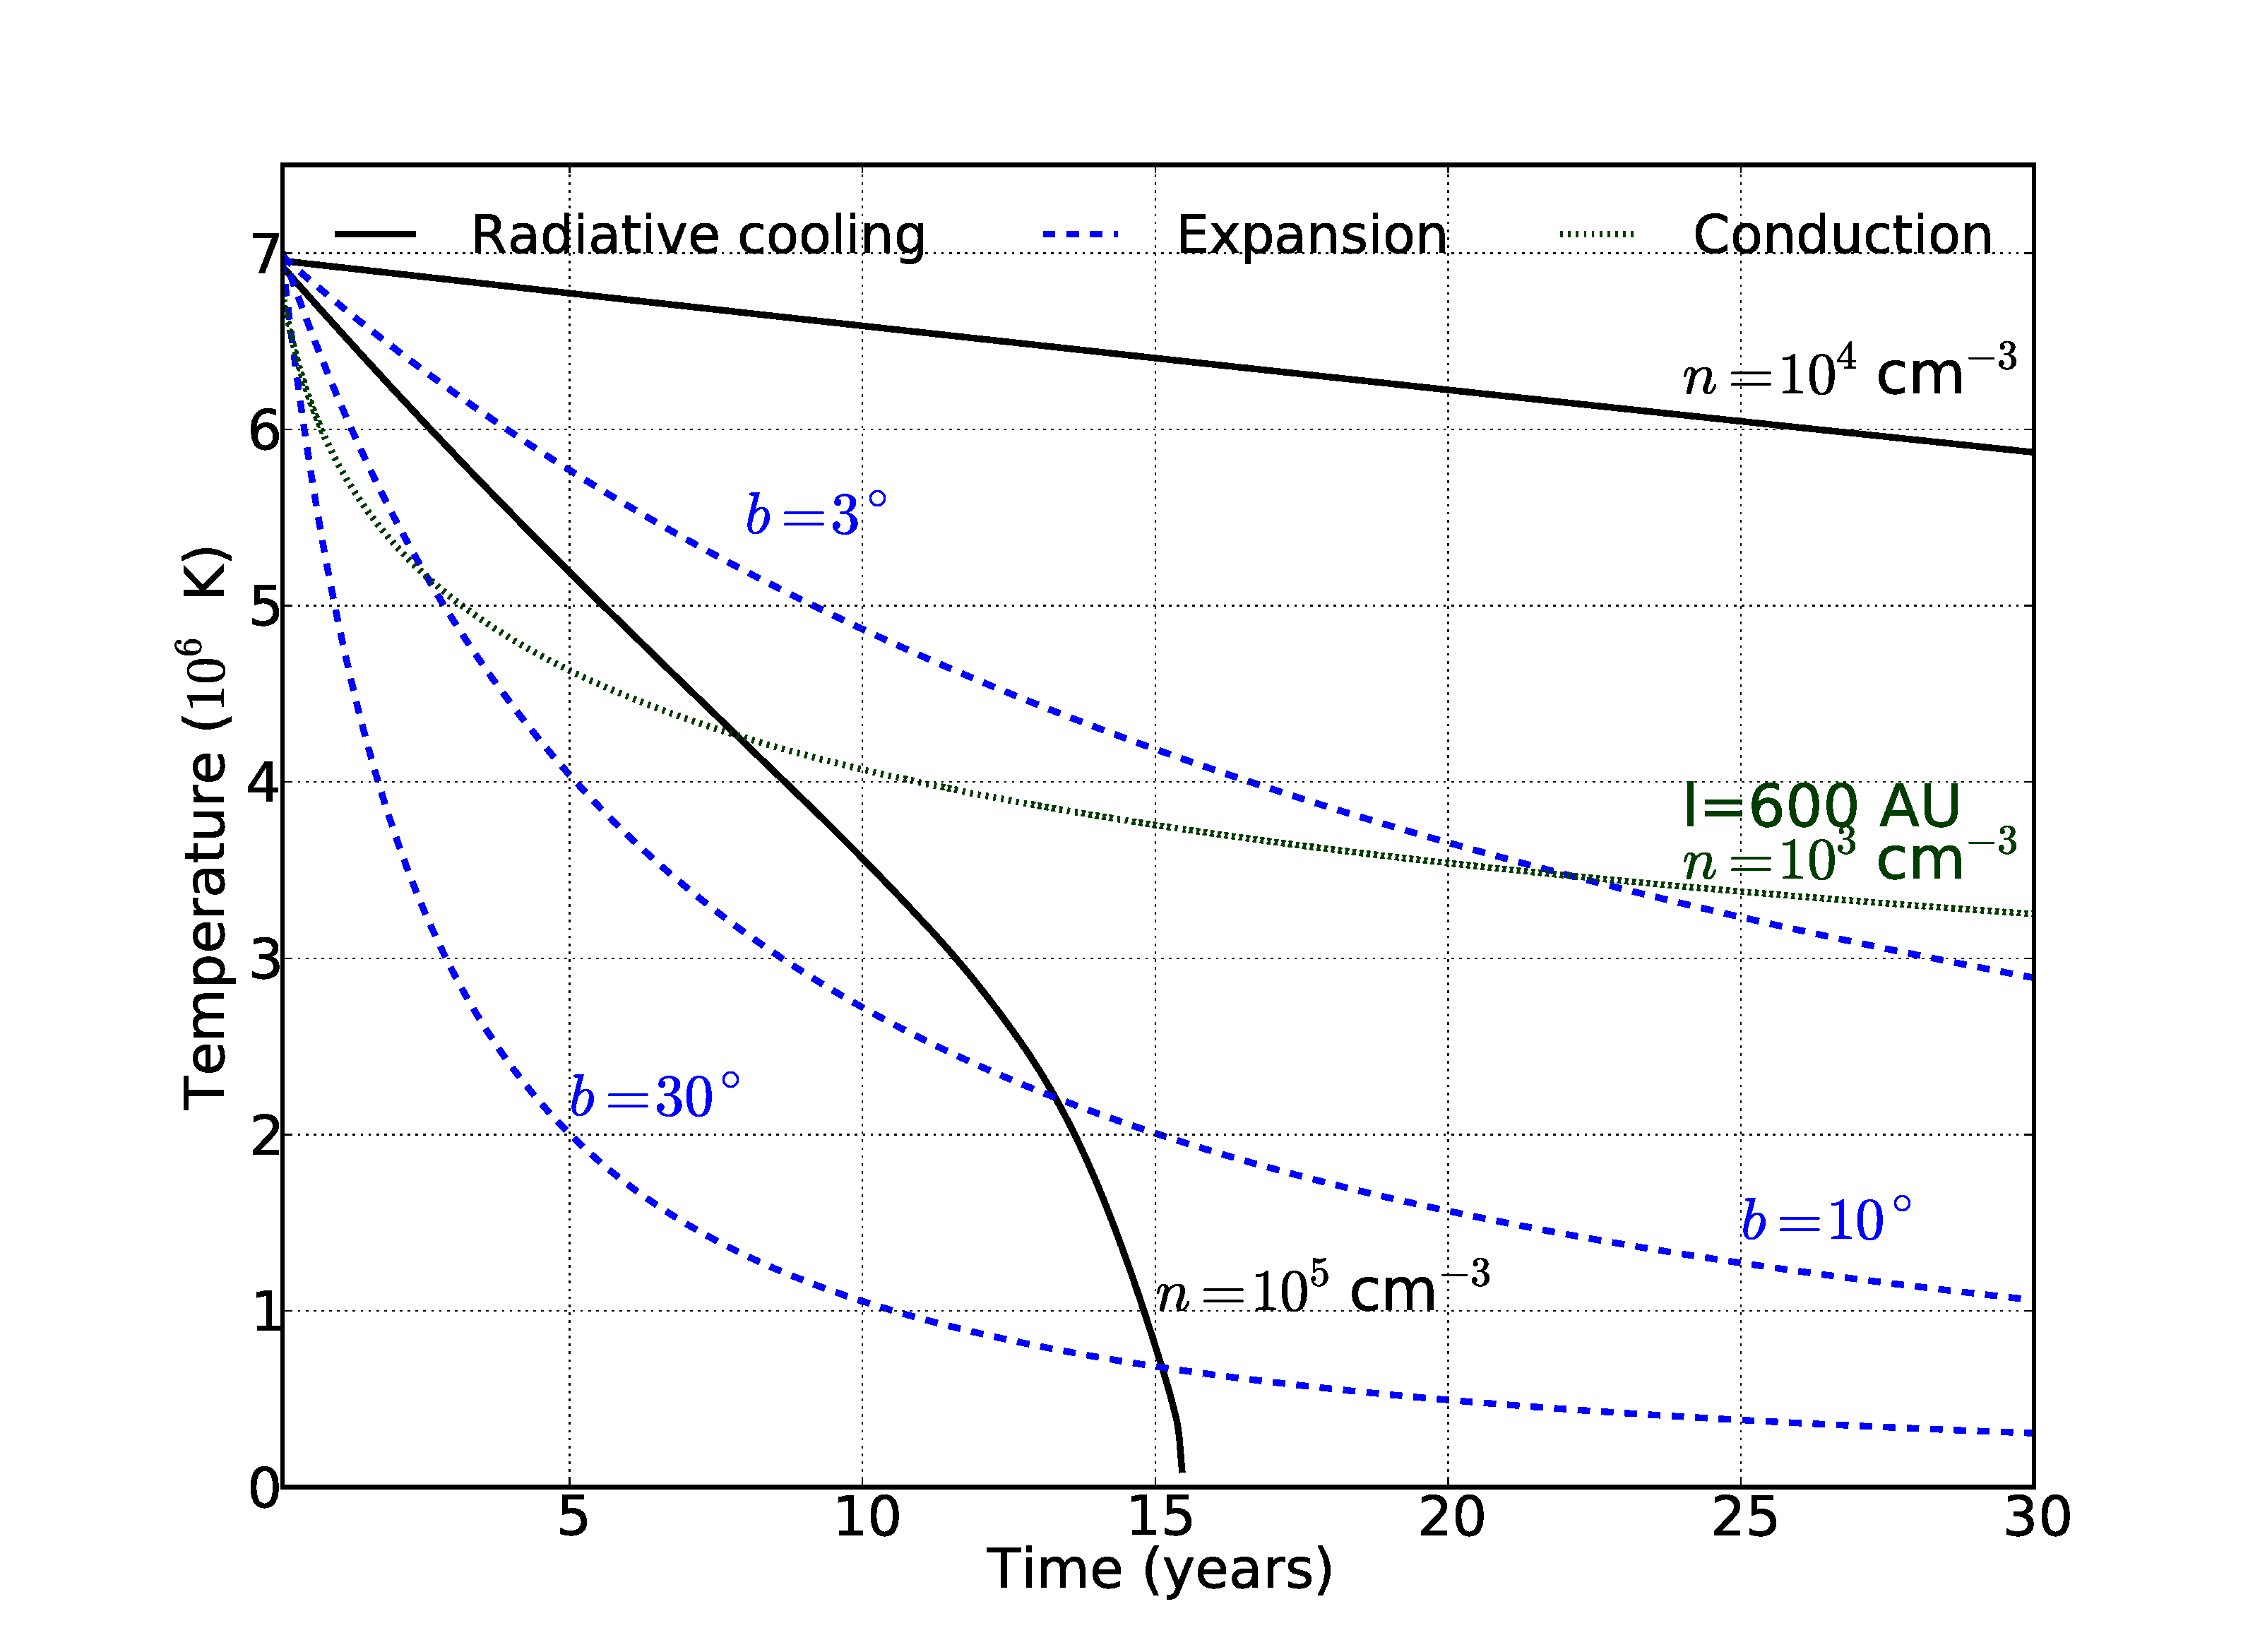
\includegraphics[width=0.49\textwidth]{figures/cool.eps}
   \caption{Cooling curves for the different cooling processes. Parameters of the models are labeled (density: $n$, opening angle: $b$, cooling length: $l$). \label{fig:cooling}}
\end{figure}


\subsubsection{Adiabatic cooling\label{sect:aCooling}}
Protostellar jets usually show an approximately conical structure at some distance from the driving sources so that the flow expands mainly perpendicular to the jet axis.
In the limit of adiabatic cooling
\begin{equation}
T\,V^{\gamma-1} = \mbox{const}
\end{equation}
holds. Since we do not observe local temperatures, we have to average the temperature, weighted by density\footnote{Note that $EM=n^2\,V=n\,N$ with a constant number of particles $N$ in each cell.}, over the volume used to measure the temperature. We use the following approximation for the volume of the plasma cell
\begin{equation}
V=\pi l\left(r_0+r\tan b \right)^2\,,
\end{equation}
where $r(t)=v\cdot t$ is the position along the jet axis measured from the initial distance, while $r_0=0.25\arcsec$ is the initial jet radius at this position and $2\cdot b$ the opening angle ($l$ is the length of the cell along the jet axis).
The initial cross-section is fixed and the temperature decrease depends only on the position along the outflow.
From the size of the Mach disk about 10\arcsec~ from the driving sources, we estimate an opening angle of $3$\,--\,$10^\circ$ for the flow, where the separation of the working surface and the Mach disk argues for values closer to $3^\circ$.
Different outflow velocities would change the curve for the expansion cooling in Fig.~\ref{fig:cooling} but would not lead to another spatial temperature structure, because the dependence on $v$ cancels out in the equations.

As described by \citet{Guedel_2008}, the expansion additionally reduces the density of the emitting plasma and thereby lowers the number of emitted photons more strongly than expected on the basis of the temperature decrease alone. For a consistency check, we calculated the expected number of photons at 3.5\arcsec~ from the driving sources from the ratio of the emission measures at 0.5\arcsec~ and 3.5\arcsec~ and the drop in temperature. Assuming constant absorption, we expect a drop in photon number by approximately a factor of about 6 from 0.5\arcsec~ to 3.5\arcsec~ for an opening angle of 3$^\circ$, which is approximately compatible with the observed value. The larger opening angle of 10$^\circ$ would reduce the photon number more strongly, i.e., the combination of the temperature and  density decrease reduces the expected photon number by about 200 for the same distance.


\subsubsection{Radiation cooling}
We solved eq.~\ref{eq:cool} using the cooling function of Chianti version~6.0 \citep{Dere_1997,Dere_2009} assuming half solar metallicity.
Figure~\ref{fig:cooling} shows two cooling curves for radiative cooling. According to eq.~\ref{eq:cool}, the cooling time depends linearly on the density. It is clear that radiative cooling does not contribute significantly to the cooling as long as the density does not exceed $n\approx10^4\,$cm$^{-3}$.

\subsubsection{Conductive cooling}
Magnetic fields are essential for the launching of jets, but even at greater distances, small magnetic fields ($\sim 100\,\mu$G) influence the jet dynamics \citep[][]{Hartigan_2007}. They can also strongly suppress heat conduction perpendicular to the field lines even for weak fields \citep[$\sim 1\mu\;$G, see eq. 5-53 in ][]{Spitzer_1962}. In the presence of turbulent magnetic fields, heat conduction might be suppressed by about two orders of magnitude or even enhanced relative to the Spitzer value \citep[e.g.][]{Narayan_2001,Cho_2003,Lazarian_2006} depending on the scale of the turbulence. We regard it as plausible that heat conduction works most efficiently along the jet axis while it is suppressed by some kind of magnetic field
perpendicular to the jet axis. The Spitzer value for the heat conduction assumes an ionized plasma, which might not be entirely true throughout the jet, however, a considerable amount of ionized material should be present close to the X-ray emitting plasma.
Given these uncertainties, we estimate conductive cooling by
\begin{eqnarray}
\tau&=&2.6\times10^{-9}\frac{n l^2}{T^{5/2}} \,\mbox{s}\\
    &\approx& 52 \left(\frac{n}{1000\,\mbox{cm}^{-3}}\right) \left(\frac{l}{210\,\mbox{AU}}\right)^2 \left( \frac{T}{3\times10^6\,\mbox{K}}\right)^{-5/2}\,\mbox{years}
\end{eqnarray}
given in \citet{Orlando_2005}. We show in Fig.~\ref{fig:cooling} a cooling curve by numerically integrating the conductive cooling for a fixed density $n$ and for
cylindrical geometry ($V\approx A\cdot l$).
The effect of the conductive cooling depends on the density of the plasma and on the temperature gradient, i.e., on the cooling length (we assumed 600\,AU for a temperature decrease from 0.6\,keV to 0.1\,keV). The curve shown in Fig.~\ref{fig:cooling} is intended to give a rough impression of this effect and we caution that the provided estimate for the conductive cooling might be off by orders of magnitude in some scenarios, e.g., for turbulent magnetic fields.

\subsubsection{Summary of cooling processes}
From Fig.~\ref{fig:cooling} it is clear that cooling by expansion dominates over radiation. Whether conduction is important depends on the density, the temperature gradient and the magnetic field configuration. When no heat is transferred perpendicular to the jet axis, we expect adiabatic cooling to dominate. We will therefore focus on that cooling process in the following.



{\color{blue}Sabina
3D view based on Ustamujic et al. MHD model}



\begin{figure}[t]
\centering

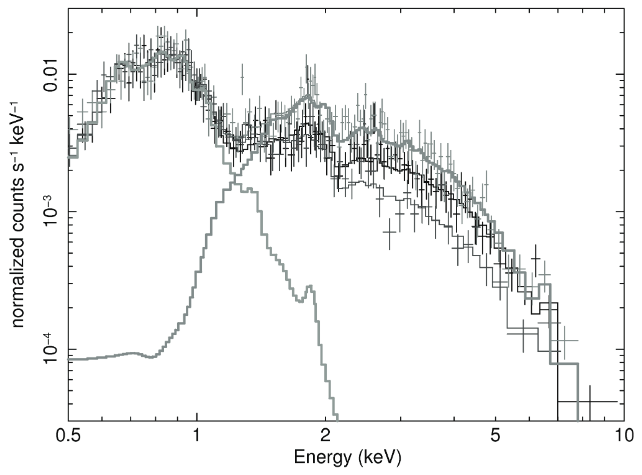
\includegraphics[height=6cm]{figs/tax}
% % %
\caption{X-ray spectrum of DG~Tau showing the two absorber nature. From \citet{}. \label{fig:tax}}
\end{figure}



\begin{figure}[t]
\centering

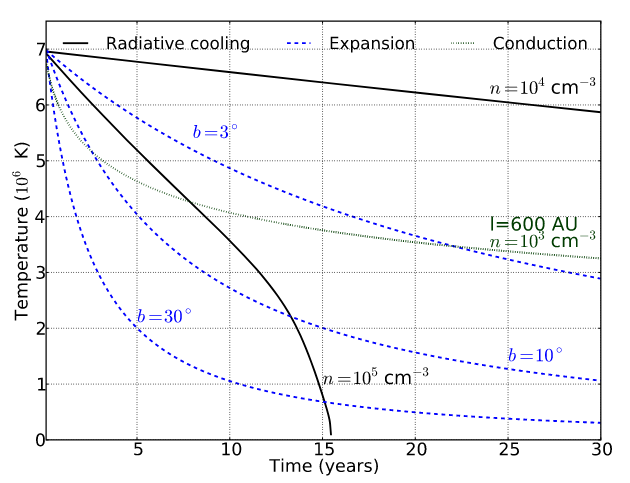
\includegraphics[height=6cm]{figs/cooling}
% % %
\caption{Cooling of an expanding, X-ray emitting plasma. \label{fig:cooling}}
\end{figure}


{\color{blue}Sabina
Stationary X-ray emission, HH objects

Collimation by the rotating magnetic field or wind pressure

Bonito et al? (HMG: Not a big fan of the setup wit ha ``nozzle'' at the disk which then leads to the diamond shock, but they are often cited and instructuve picture)

Lab work in here, too?
}


\begin{figure}[t]
\centering

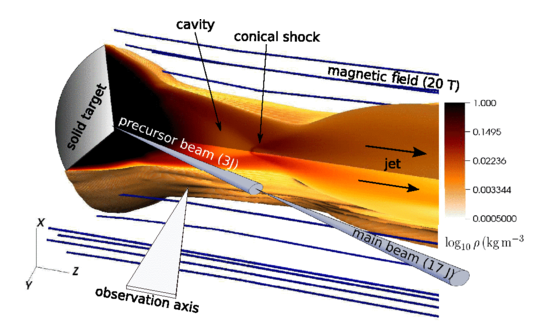
\includegraphics[height=6cm]{figs/lab}
% % %
\caption{Lab experiment. From \citet{PhysRevLett.119.255002}. \label{fig:lab}}
\end{figure}


\subsection{Connection to other obs}
{\color{blue}Christian

UV obs (DG Tau jet), [Fe II] monitoring, Liu [Ne III]?

Jet rotation

}


\section{Outlook}
{\color{blue}(2 pages) [all]

Athena, Lynx, Arcus (figures will be new, Moritz can make for Lynx, Arcus)(?)
}


\section{Instruction - DELETE}

\vspace{0.3cm}

{\bf Key-points to have in mind}:
\begin{enumerate}
\item The {\it Handbook of X-ray and Gamma-ray Astrophysics} is aiming to publish a work of tertiary literature, which provides easily accessible, digested and established knowledge derived from primary or secondary sources in the particular field. Therefore, your contribution should be clear and concise and be a comprehensive and up-to-date overview of your topic.
\item Length of text: every chapter normally consists of about 10,000-20,000 words (excluding figures and references), which would be about 20-40 typeset pages. However, this is not a rigid rule and it is something to discuss with the Section Editors of the Section of the chapter.
\item Colored figures are welcome in any standard format (jpg, tif, ppt, gif). If possible please provide the original figure in high resolution (300 dpi minimum). {\color{red}\bf Please do not forget to obtain permission in case the figure is from a published article}. For journals like ApJ, PRD, PRL, etc. you do not need the permission if you are an author of the article of the original figures, but for most journals you need the permission even if you are the author of those figures. However, if you create a new figures with minor changes, you can claim it is a new figure and you do not need any permission.
\end{enumerate}


\vspace{0.5cm}

{\bf Submission}:

\vspace{0.1cm}

{\color{red} \bf Please submit source files, compiled pdf file of the chapter, and figure permissions through the Meteor system.}

\vspace{0.5cm}

{\bf arXiv policy}:

\vspace{0.1cm}

{Authors can post their chapter on arXiv if they wish to do it. In the comment field, please write something like ``Invited chapter for {\it Handbook of X-ray and Gamma-ray Astrophysics} (Eds. C. Bambi and A. Santangelo, Springer Singapore, expected in 2022)''. After the publication of the chapter, you may add the DOI on the arXiv page.}



\section{Cross-References \textit{(if applicable)}}
Include a list of related entries from the handbook here that may be of further interest to the readers.

% bibs will be alphametically ordered. I think that's what they want.
% if not, see: https://tex.stackexchange.com/questions/312819/problem-with-springer-bibliography-stylespbasic-natbib
\bibliographystyle{spbasic}
\bibliography{bib.bib}

\end{document}
